\documentclass[landscape,footrule]{foils}
\usepackage[lecture-serie]{foiltex-extra}
\usepackage{crysymb}
\usepackage{graphics}
\usepackage[pdftex]{graphicx} 




\newcommand{\lserie}{LTAT.02.004 Machine Learning II}
\newcommand{\lecture}{Normal distribution and affine projections}
\newcommand{\ldate}{March 26, 2019}
\newcommand{\lauthor}{Sven Laur}
\newcommand{\linst}{University of Tartu}
\graphicspath{{./illustrations/}}

\renewcommand{\VAR}{\mathbf{Var}}
\DeclareMathOperator{\diag}{diag}

\newcommand{\leqm}{\ \leq_m}


\newcommand{\bigvskip}{\vskip 2em}
\newcommand{\lastline}{\vspace*{-2ex}}
\newcommand{\spreadappart}{\vspace*{\fill}}


\newcommand{\EVPOS}{\textcolor{red}{\mathsf{evidence}^+}}
\newcommand{\EVPOSI}{\textcolor{red}{\mathsf{evidence}^+_i}}
\newcommand{\EVNEG}{\textcolor{blue}{\mathsf{evidence}^-}}

\newcommand{\COV}{\mathbf{Cov}}
\begin{document}
\titlefoil


\middlefoil{Univariate normal distribution}

\foilhead[-1cm]{Probability density function}

\illustration[scale=0.5]{pdf_vs_pmf}
\textbf{Definition.}
A real-valued random variable $X$ comes from a continuous distribution with \emph{a probability density function} $p:\RR\to\RR^+\cup\set{0}$ if the following limit exists for any $x\in\RR$:
\begin{align*}
p(x)=\lim_{\Delta x \to 0^+} \frac{\pr{x -\Delta x \leq X\leq x+\Delta x}}{2\cdot \Delta x}\enspace.
\end{align*} 


\foilhead[-1cm]{Probability mass function}

\illustration[scale=0.5]{pdf_vs_pmf}

\textbf{Definition.}
A real-valued random variable $X$ comes from a discrete distribution with \emph{a probability mass function} $p:\RR\to\RR^+\cup\set{0}$ defined as 
\begin{align*}
p(x)=\pr{X=x}=\lim_{\Delta x \to 0^+} \pr{x-\Delta x \leq X\leq x+\Delta x}
\end{align*}  
if there exist a sequence $(x_i)_{i=1}^\infty$ such that $p(x_1)+\ldots+p(x_i)+\ldots =1$.


\foilhead[-1cm]{Standard normal distribution }

\illustration[scale=0.5]{standard_normal_distribution}

Standard normal distribution $\NNN(\mu=0,\sigma=1)$ is a continuous distribution with a probability density function 
\begin{align*}
p(x)=\frac{1}{\sqrt{2\pi}}\cdot\exp{-\frac{x^2}{2}}
\end{align*}
The mean value $\mu=0$ and variance $\sigma^2=1$ for this distribution.


\foilhead[-1cm]{Univariate normal distribution}

\textbf{Definition.}
A random variable $y$ is distributed according to a normal distribution $\NNN(\mu=a,\sigma=b)$ if it can be expressed 
\begin{align*}
y=bx+a
\end{align*}
where $x$ is distributed according to standardised normal distribution~$\NNN(0,1)$. \vspace*{1cm}

The corresponding probability density functions is
\begin{align*}
p[y|\mu,\sigma]=\frac{1}{\sqrt{2\pi}\sigma}\cdot\exp{\frac{(x-\mu)^2}{2\sigma^2}}
\end{align*}
and the mean value $\mu$ and variance $\sigma^2$ for this distribution.


\foilhead[-1cm]{Density derivation}

\centerline{
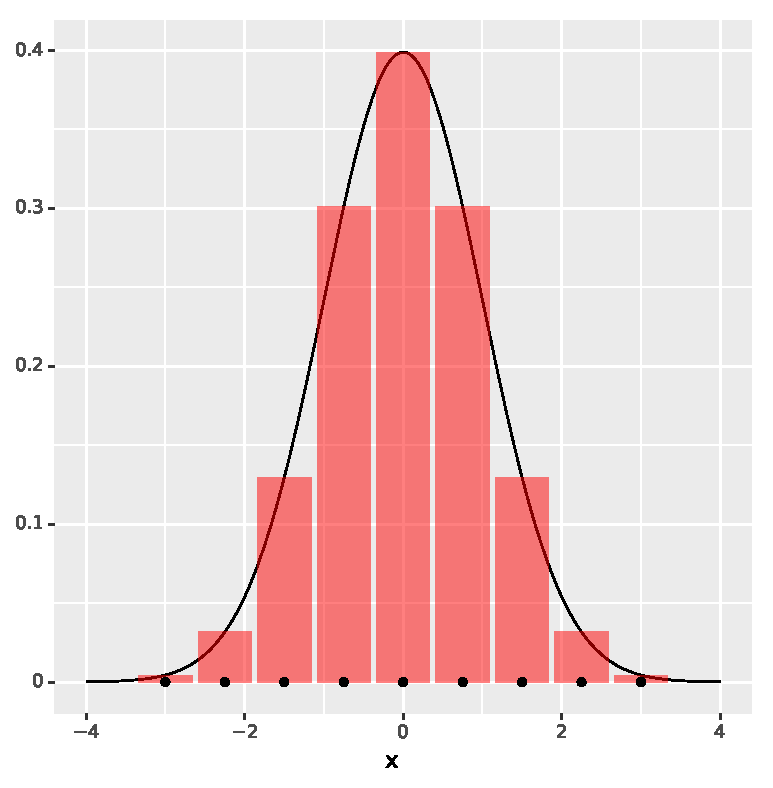
\includegraphics[scale=0.5]{1d_source_distribution}\hspace*{1cm}
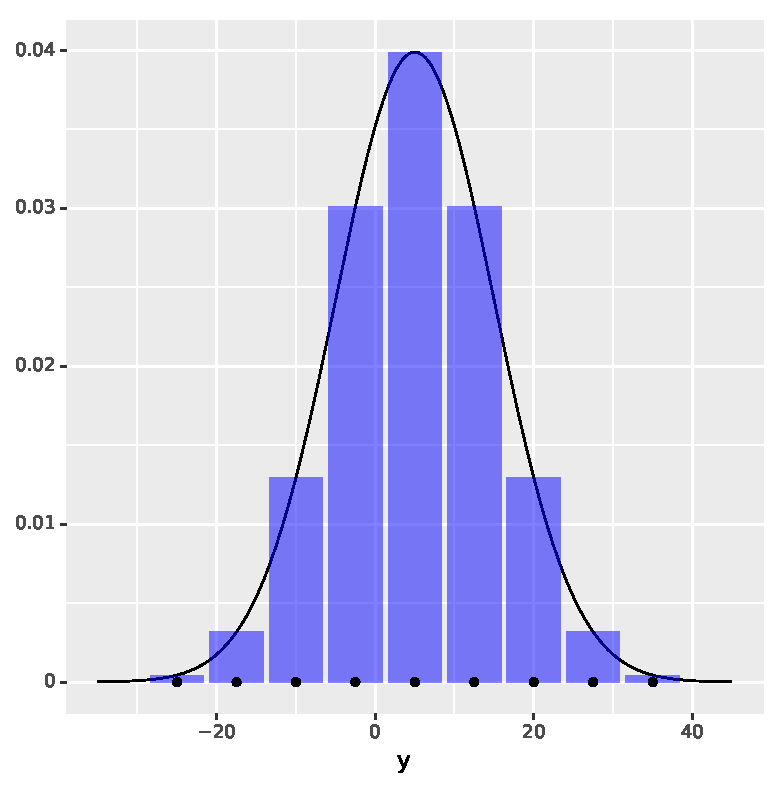
\includegraphics[scale=0.5]{1d_target_distribution}}

Let $y=ax + b$ the the relation between densities 
\begin{align*}
p_x(x)=\sigma\cdot p_y(y)
\end{align*}
follows form the fact that areas of red and blue columns must be the same.



\middlefoil{Multivariate normal distribution}


\foilhead[-1cm]{White Gaussian noise}

\illustration[scale=0.4]{white_gaussian_noise}
\vspace*{-1.0cm}

\textbf{Definition.} A random vector $X_1,\ldots, X_n$ is a standard normal random vector if all of its components are independent and and $X_i\sim \NNN(0,1)$.
\begin{triangles}
\item The density can be computed based on independence:
\begin{align*}
p(x_1,\ldots,x_n)=p(x_1)\cdots p(x_n)=\frac{1}{(2\pi)^{n/2}}\cdot\mathsf{exp}\Biggl(-\frac{x_1^2+\cdots+x_n^2}{2}\Biggl)\enspace.
\end{align*}
\end{triangles}

\foilhead[-1cm]{Scaling and shifting}

By shifting and scaling the source distribution $\NNN(\vec{0},I)$ we can obtain some other instances of multivariate normal distribution.
\vspace*{-1cm}

\begin{center}
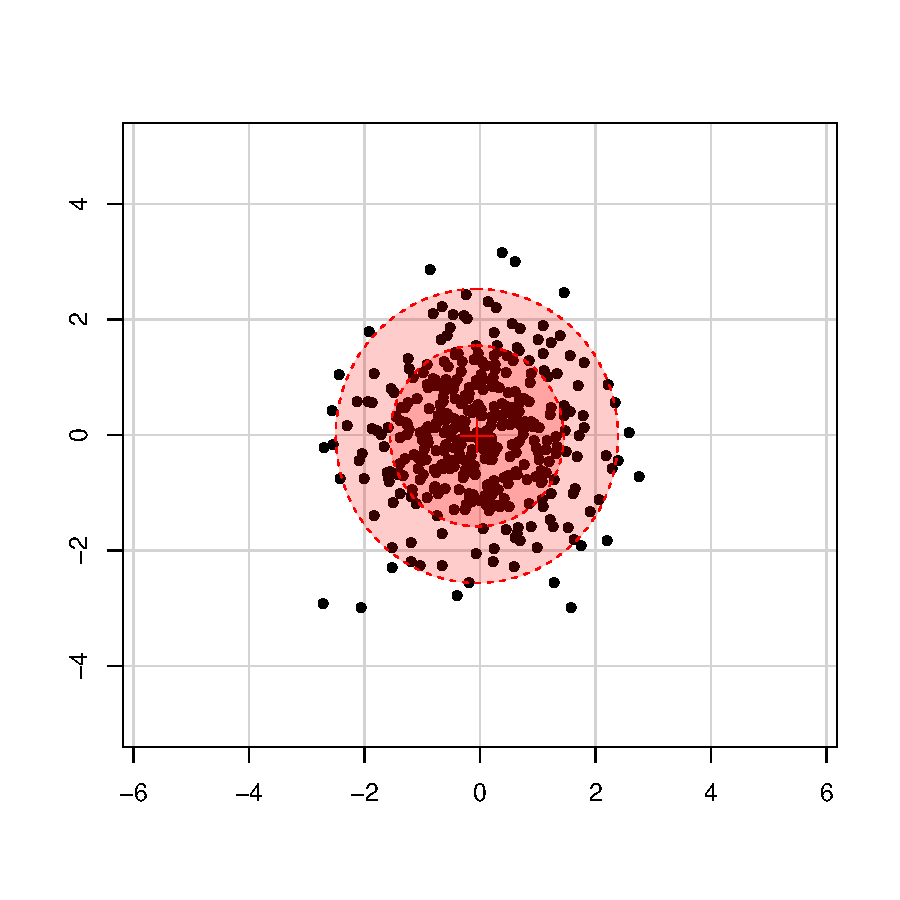
\includegraphics[scale=0.65]{source-distribution.pdf}
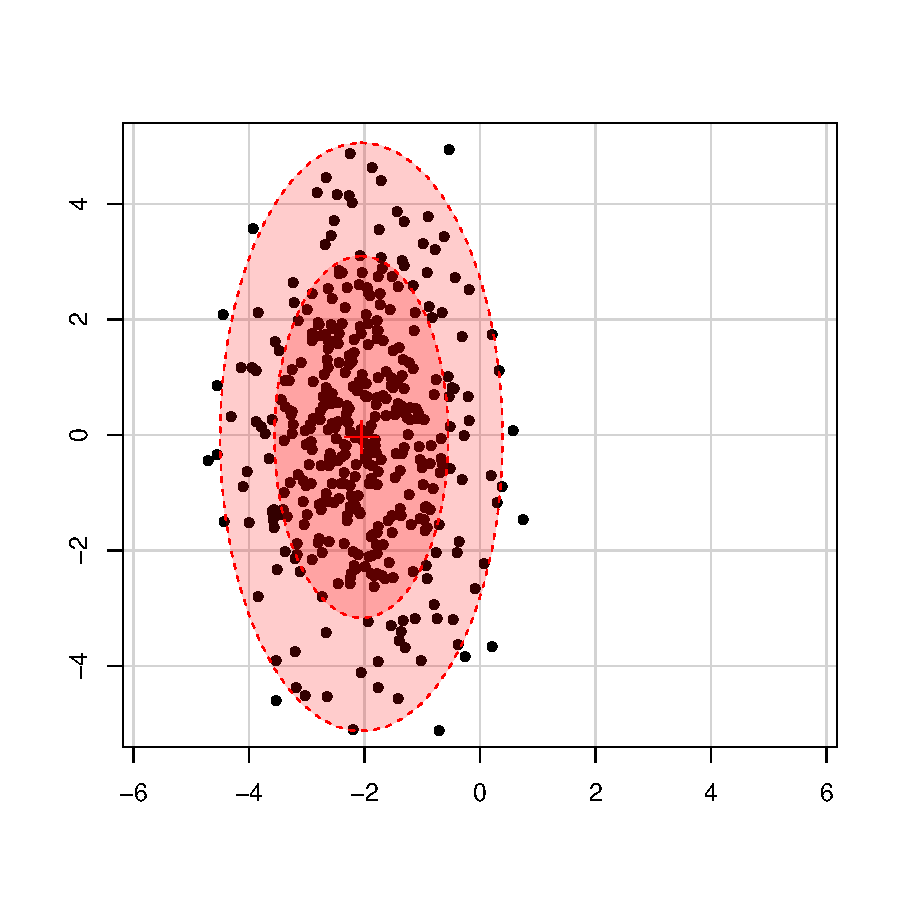
\includegraphics[scale=0.65]{scaled-distribution.pdf}
\end{center}\vspace*{-10cm}





\foilhead[-1cm]{Necessity of rotations}

As the choice of coordinate axis is sometimes arbitrary, there must be other ways to form a normal distribution -- rotations of coordinate axis.\vspace*{-1cm}  

\begin{center}
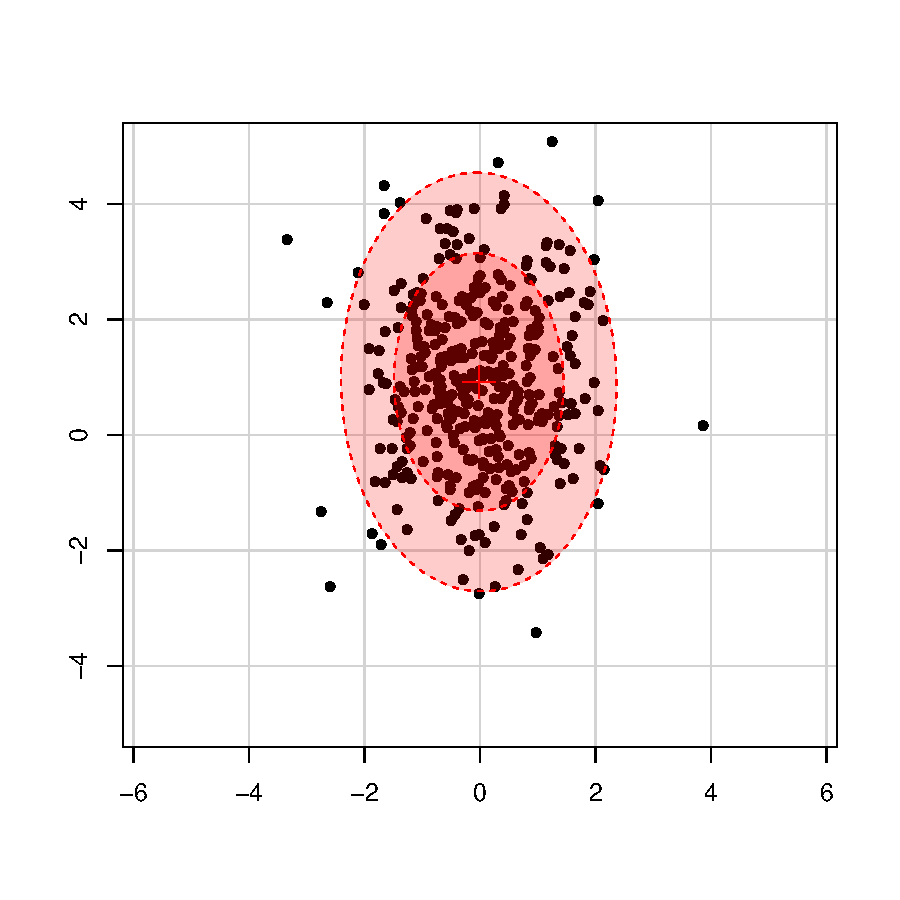
\includegraphics[scale=0.65]{two-dimensional-normal-distribution-i.pdf}
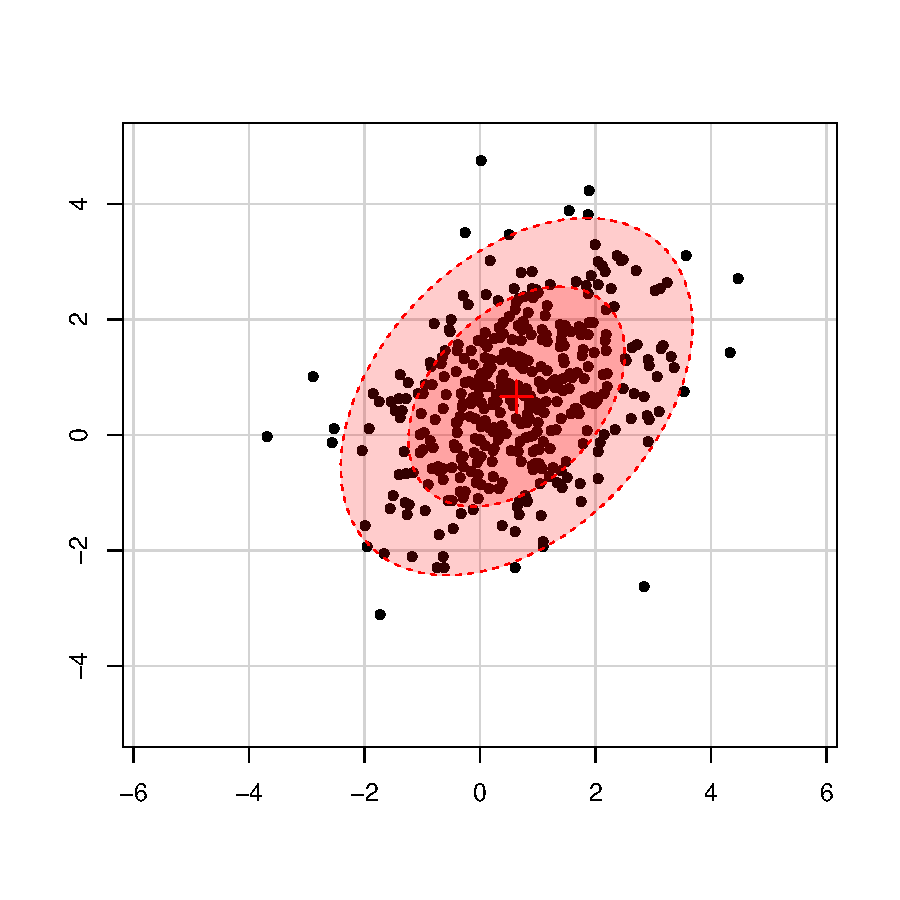
\includegraphics[scale=0.65]{two-dimensional-normal-distribution-ii.pdf}
\end{center}\vspace*{-1cm}

Any affine transformation can be expressed as scaling, rotating and shifting.




\foilhead[-1cm]{Affine transformations}

Let $\vec{x}$ be standard normal random vector and let $\vec{y}$ be obtained the scaling,  translation and rotation of the coordinate plane.

Then we can express $\vec{x}$ and $\vec{y}$ in terms of an affine transformation
\begin{align*}
  \vec{y}&=A\vec{x}+\vec{\mu} \enspace,\\
  \vec{x}&=A^{-1}(\vec{y}-\vec{\mu}) \enspace.
\end{align*}

\textbf{Observation.}
Affine transformations are closed with respect to composition, i.e., applying two affine transformations yields a new affine transformation. \vspace*{2ex}

\textbf{Remark.} Not all affine transformations are invertible.\lastline


\foilhead[-1cm]{What is density in 2D?}


Recall that density assigns probability to small enough regions $\RRR$:
\begin{align*}
\pr{\begin{aligned}
 & x_1^*\gets \NNN(0,1):x_1\leq x_1^*\leq x_1+\Delta x_1\\ 
 & x_2^*\gets \NNN(0,1):x_2\leq x_2^*\leq x_2+\Delta x_2
\end{aligned}}= p(x_1,x_2)\cdot\underbrace{\Delta x_1\Delta x_2}_S +\, \varepsilon
\end{align*}
where $\varepsilon=o(\Delta x_1\cdot\Delta x_2)$ in the process $\Delta x_1\to 0$ and $\Delta x_2\to 0$.\vspace*{1cm}

\textbf{Remark.} Regions $\RRR$ do not have to be rectangular as long as:
\begin{triangles}
\item The area $S(\RRR)$ of a region can be computed.  
\item Probability can be assigned to the region $\RRR$ and its scalings.
\end{triangles}
Then $\varepsilon=o(S)$ when we rescale the region $\RRR$ around the point $(x_1,x_2)$.


\foilhead[-1cm]{Density recalibration}

Any affine transformation changes a square grid into parallelograms. \vspace*{-1cm}
\begin{center}
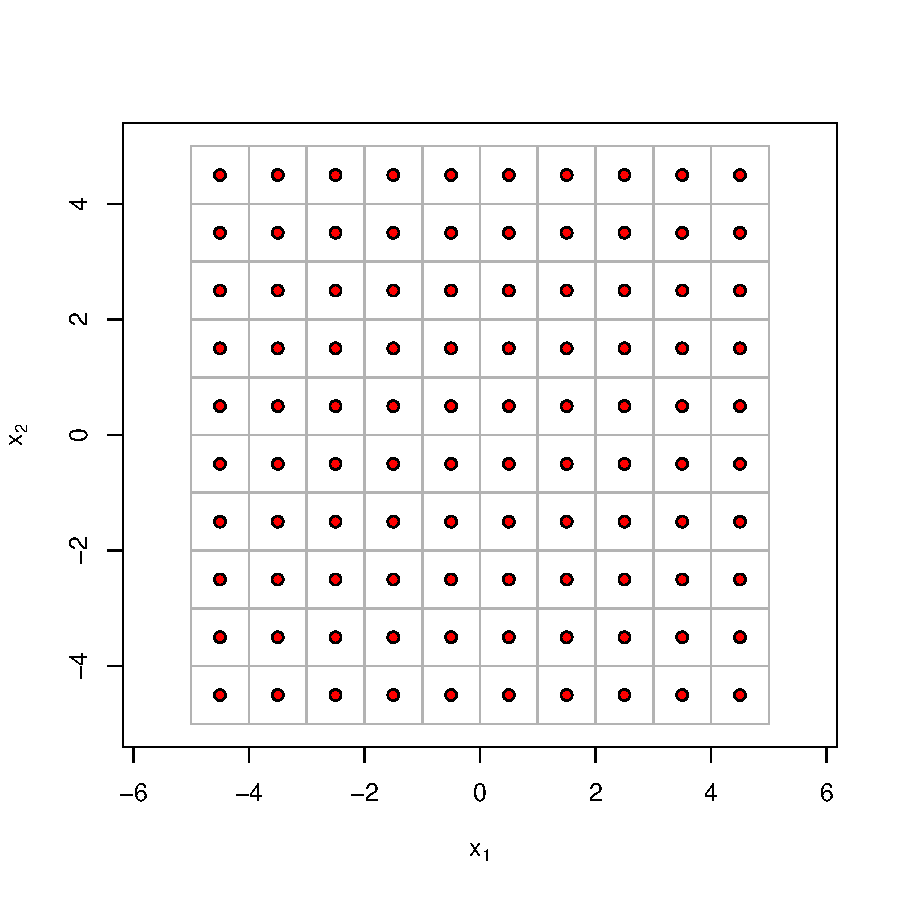
\includegraphics[scale=0.55]{original-grid.pdf}
\raisebox{4.0cm}{$\quad\xrightarrow{\vec{y}=A\vec{x}+\vec{\mu}}\quad$}
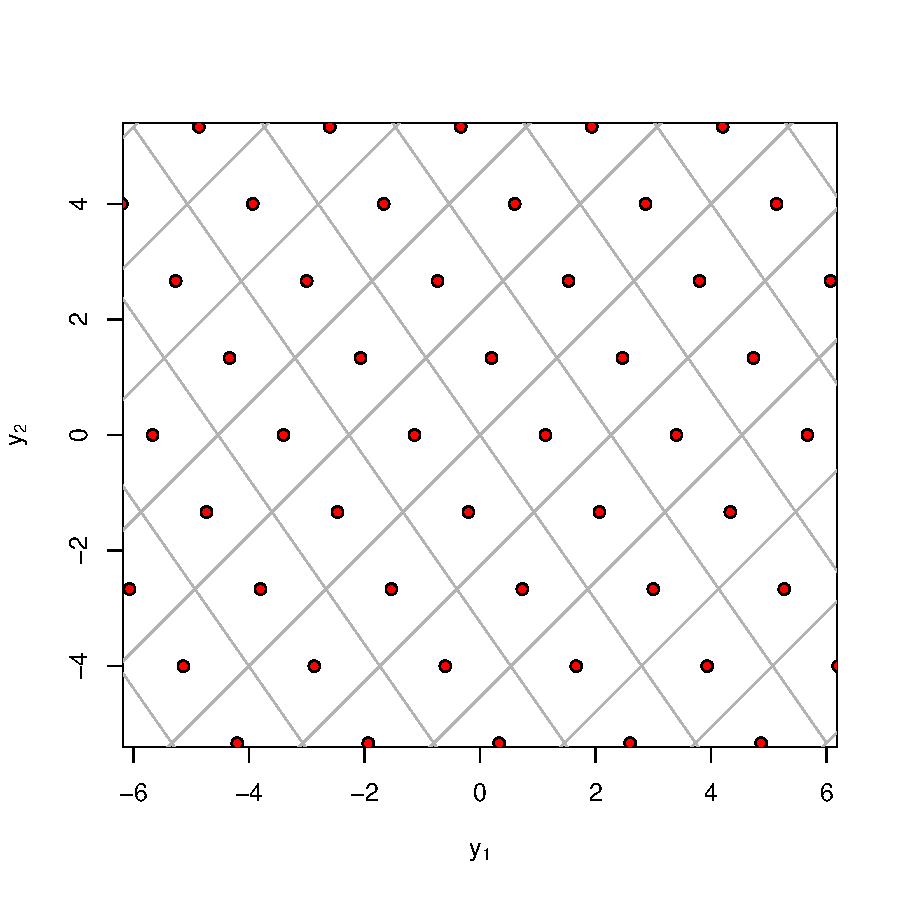
\includegraphics[scale=0.55]{transformed-grid.pdf}
\end{center}\vspace*{-1cm}

As a result, the area of the regions is different on the left and on the right:
\begin{align*}
p(x_1,x_2)\cdot S_1\approx q(y_1,y_2)\cdot S_2\qquad\Longrightarrow\qquad q(y_1,y_2)={\frac{S_1}{S_2}}\cdot p(x_1,x_2) 
\end{align*}
Fortunately, the ratio between areas are constant over the entire plane!\lastline

  
\foilhead[-1cm]{Density of two-variate normal distribution}

\enlargethispage{1cm}
The density of $(x_1,x_2)$ pairs can be computed based on independence:
\begin{align*}
p(x_1,x_2)=p(x_1)\cdot p(x_2)=\frac{1}{2\pi}\cdot\mathsf{exp}\Biggl(-\frac{x_1^2+x_2^2}{2}\Biggl)\enspace.
\end{align*}
\vspace*{-3ex}

To estimate density $q(y_1,y_2)$, we must find the corresponding $(x_1,x_2)$:
\begin{align*}
 \vec{y}=A\vec{x}+\vec{\mu}\quad\Leftrightarrow\quad \vec{x}=A^{-1}(\vec{y}-\vec{\mu})\enspace. 
\end{align*}
Thus we get \vspace*{-2ex}
\begin{align*}
q(y_1,y_2)&=\frac{S_1}{S_2}\cdot\frac{1}{2\pi}\cdot
\exp{-\frac{(\vec{y}-\vec{\mu})^T A^{-T}A^{-1}(\vec{y}-\vec{\mu})}{2}}\\
&=\frac{1}{\sqrt{\det(\Sigma)}}\cdot\frac{1}{2\pi}\cdot
\exp{-\frac{(\vec{y}-\vec{\mu})^T \Sigma^{-1}(\vec{y}-\vec{\mu})}{2}}\enspace.
\end{align*}

 

\foilhead[-1cm]{Illustrative example}
 
\begin{center}
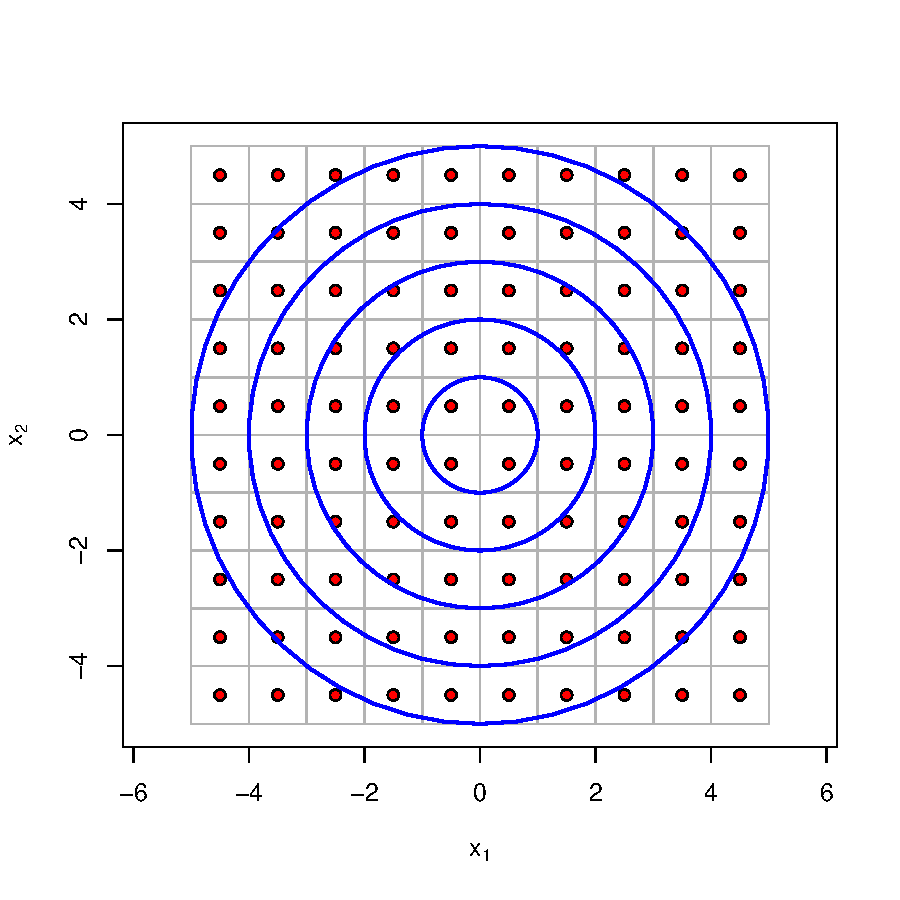
\includegraphics[scale=0.55]{original-contours.pdf}
\raisebox{4.0cm}{$\quad\xrightarrow{\vec{y}=A\vec{x}+\vec{\mu}}\quad$}
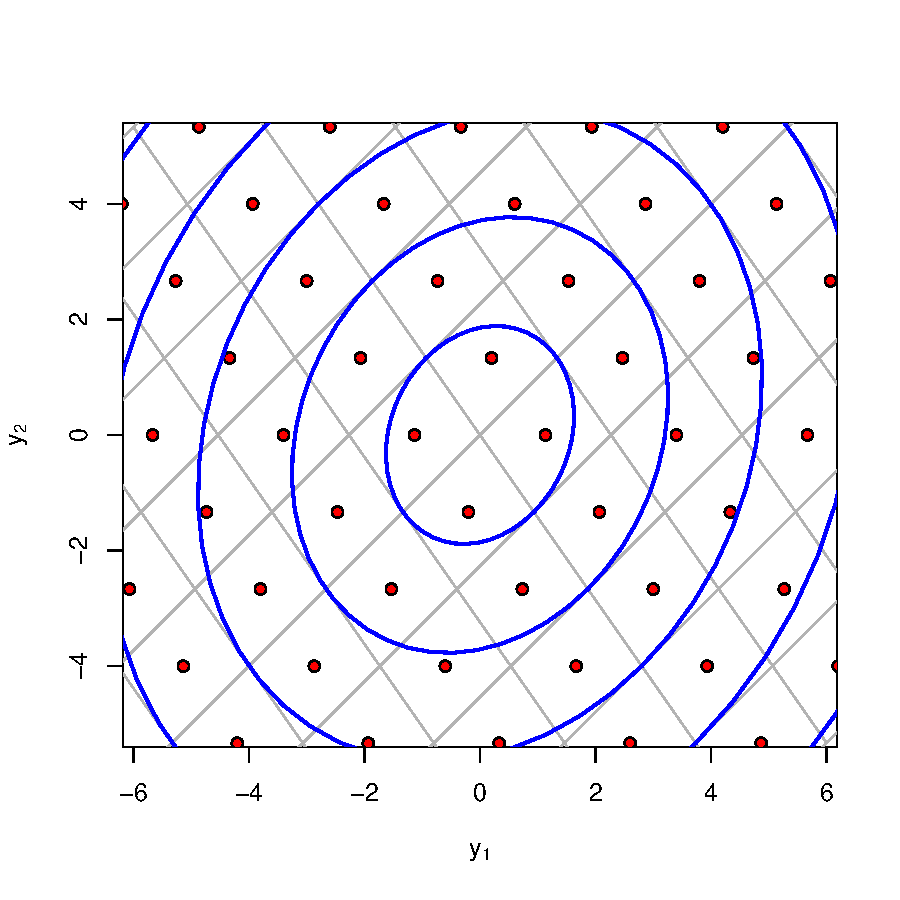
\includegraphics[scale=0.55]{transformed-contours.pdf}
\end{center}\vspace*{-0cm}

\begin{triangles}
\item Affine transformation changes the square grid into parallelograms. 
\item Affine transformation changes circular equiprobability lines into ellipses. 
\item The axes of the ellipses may intersect with the sides of parallelograms.
\end{triangles}



\foilhead[-1cm]{Generalisation to multivariate case}

If observed quantities $\vec{y}$ are generated by applying the affine transformation 
\begin{align*}
 \vec{y}=A\vec{x}+\vec{\mu}\quad\Leftrightarrow\quad \vec{x}=A^{-1}(\vec{y}-\vec{\mu})\enspace
\end{align*}
to the \emph{independent source signals} $x_1,\ldots, x_n\sim\NNN(0,1)$, then the resulting distribution is \emph{a multivariate normal distribution} with the density:
\begin{align*}
p(\vec{y})&=\frac{1}{(2\pi)^{n/2}}\cdot\frac{1}{\sqrt{\det(\Sigma)}}\cdot
\exp{-\frac{(\vec{y}-\vec{\mu})^T \Sigma^{-1}(\vec{y}-\vec{\mu})}{2}}\enspace
\end{align*} 
where $\Sigma^{-1}=A^{-T}A^{-1}$ is \emph{a positively definite symmetric matrix}.


\middlefoil{Important properties of\vspace*{1ex}\\ normal distributions}

\foilhead[-1cm]{Closeness under marginalisation}

Let $\vec{x}_{\III}=(x_i)_{i\in\III}$ be a subvector determined by the coordinate set $\III$.
Then $\vec{x}_{\III}$ is distributed according to a multivariate normal distribution as long as 
the vector $\vec{x}$ comes form a multivariate normal distribution $\NNN(\vec{\mu},\Sigma)$.

\begin{triangles}
\item Moment matching gives the parameters of the resulting distribution 
\begin{align*}
\EXP(\vec{x}_{\III})&= \EXP(\vec{x})_{\III}=\vec{\mu}_{\III} \\
\COV(\vec{x}_{\III})&=\COV(\vec{x})_{\III\times \III}=\Sigma[\III, \III]
\end{align*}
\end{triangles}

\foilhead[-1cm]{Closeness under linear combinations}

Linear combination $y=\vec{\alpha}_1^T \vec{x}_1+\vec{\alpha}_2^T\vec{x}_2$ of independent multivariate normal distributions $\vec{x}_1\sim\NNN(\vec{\mu}_1,\Sigma_1)$ and $\vec{x}_2\sim\NNN(\vec{\mu}_2,\Sigma_2)$ is also  a multivariate normal distribution.

\begin{triangles}
\item Moment matching gives the parameters of the resulting distribution 
\begin{align*}
\EXP(y)&= \vec{\alpha}_1^T\EXP(\vec{x}_1)+\vec{\alpha}_2^T\EXP(\vec{x}_2)=
\vec{\alpha}_1^T\vec{\mu}_1+\vec{\alpha}_2^T\vec{\mu}_2\\
\VAR(y)&=\COV(\vec{\alpha}_1^T \vec{x}_1) + \COV(\vec{\alpha}_2^T \vec{x}_2)\\
&=\vec{\alpha}_1^T \COV(\vec{x}_1)\vec{\alpha}_1+ \vec{\alpha}_2^T \COV(\vec{x}_2)\vec{\alpha}_2\\
&=\vec{\alpha}_1^T \Sigma_1\vec{\alpha}_1+ \vec{\alpha}_2^T \Sigma_2\vec{\alpha}_2
\end{align*}
\item Closeness under linear combinations holds also for matrix combinations. 
\end{triangles}

\foilhead[-1cm]{Closeness under conditioning}

Let $\vec{x}$ and $\vec{y}$ be related random variables. 
Let $\vec{x}|\vec{y}_*$ denote the conditional distribution of $\vec{x}$ given that a random variable $\vec{y}$ has a fixed value $\vec{y}_*$.
Then $\vec{x}|\vec{y}_*$ is distributed according to a multivariate normal distribution provided that 
 $(\vec{x},\vec{y})$ comes form a multivariate normal distribution $\NNN((\vec{\mu}_i),(\Sigma_{ij}))$

\begin{triangles}
\item Moment matching gives the parameters of the resulting distribution 
\begin{align*}
\EXP(\vec{x}|\vec{y}_*)&= \vec{\mu}_1+ \Sigma_{1,2}\Sigma_{2,2}^{-1}(\vec{y}-\vec{\mu}_2)\\
\COV(\vec{x}|\vec{y}_*)&= \Sigma_{1,1}-\Sigma_{1,2}\Sigma_{2,2}^{-1}\Sigma_{2,1}\\
\end{align*}
\end{triangles}

\middlefoil{Principal component\vspace*{1ex}\\ analysis}


\foilhead[-1cm]{Distribution reconstruction task}

\textbf{Original goal.} 
Given the set of observations $\vec{y}_1,\ldots, \vec{y}_m$ determine the affine transformation $\vec{y}=A\vec{x}+\vec{\mu}$ and original source signals  $\vec{x}_1,\ldots, \vec{x}_m$.


\textbf{Impossibility result.}
The matrix $A$ can be recovered \emph{only} up to rotations.


\begin{center}
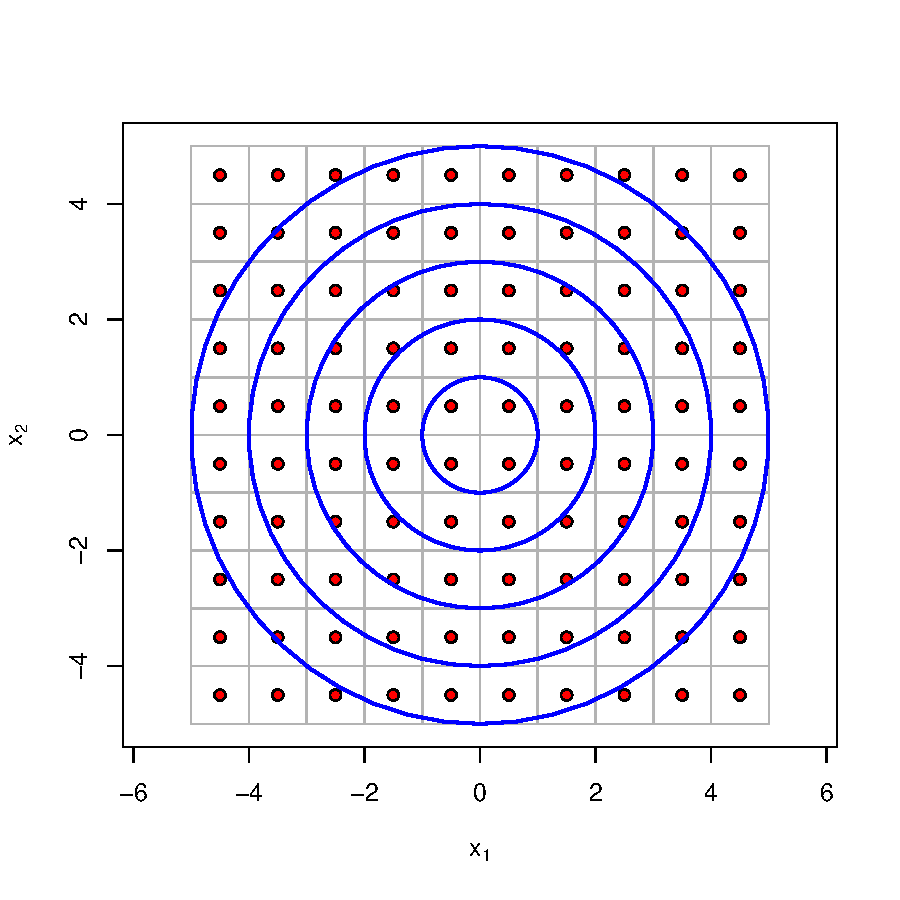
\includegraphics[scale=0.55]{original-contours.pdf}
\raisebox{4.0cm}{$\quad\xrightarrow{\vec{y}=A\vec{x}+\vec{\mu}}\quad$}
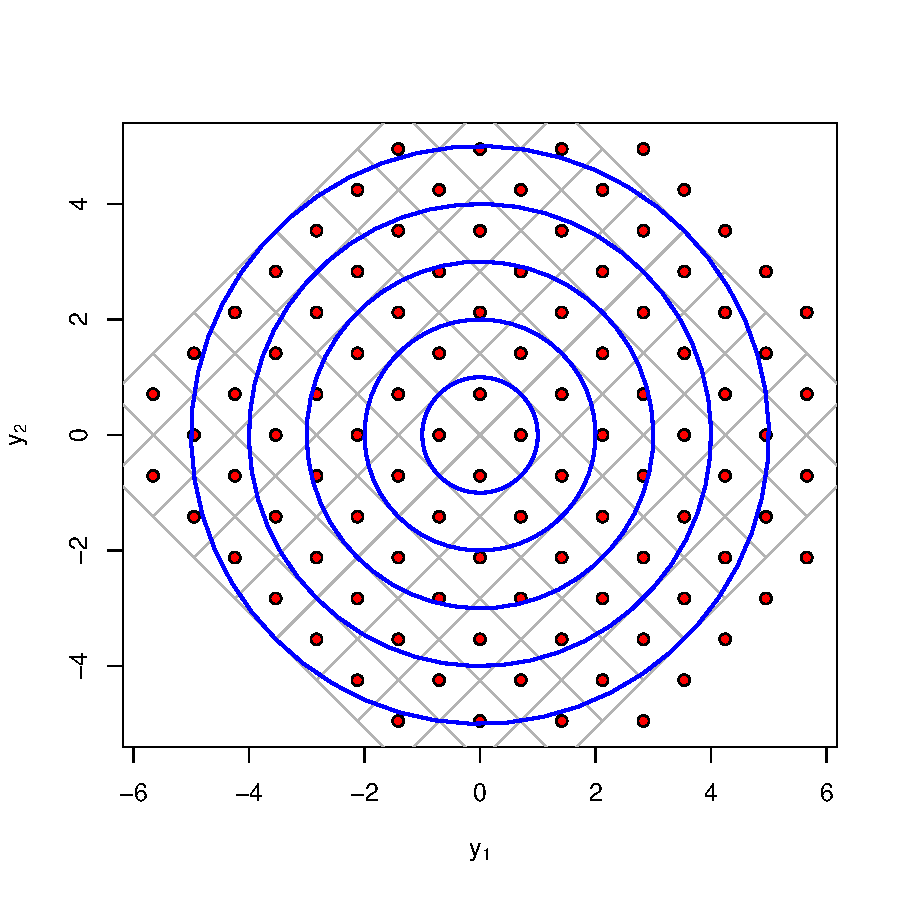
\includegraphics[scale=0.55]{rotated-contours.pdf}
\end{center}\vspace*{-1cm}



\foilhead[-1cm]{Simplified distribution reconstruction task}

\textbf{Achievable goal.}
Given the set of observations $\vec{y}_1,\ldots, \vec{y}_m$ determine the affine transformation by fixing the centre and axis of the ellipsoid.


\begin{center}
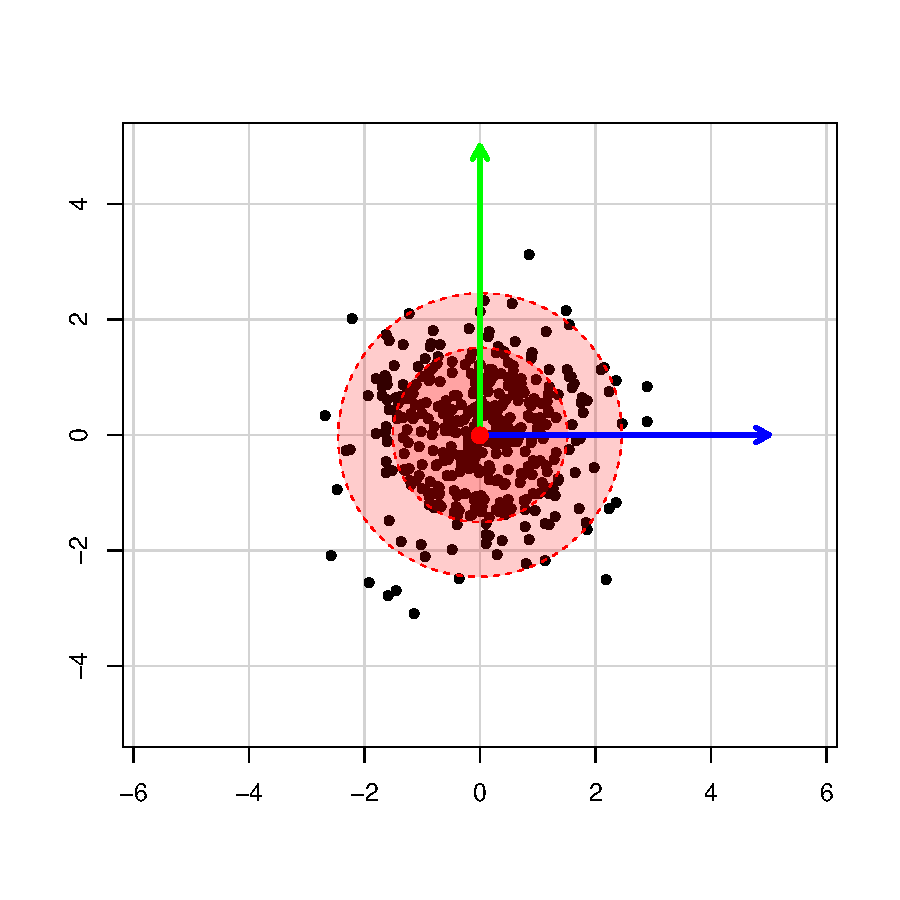
\includegraphics[scale=0.55]{source-distribution-iii.pdf}
\raisebox{4.0cm}{$\quad\xrightarrow{\vec{y}=A\vec{x}+\vec{\mu}}\quad$}
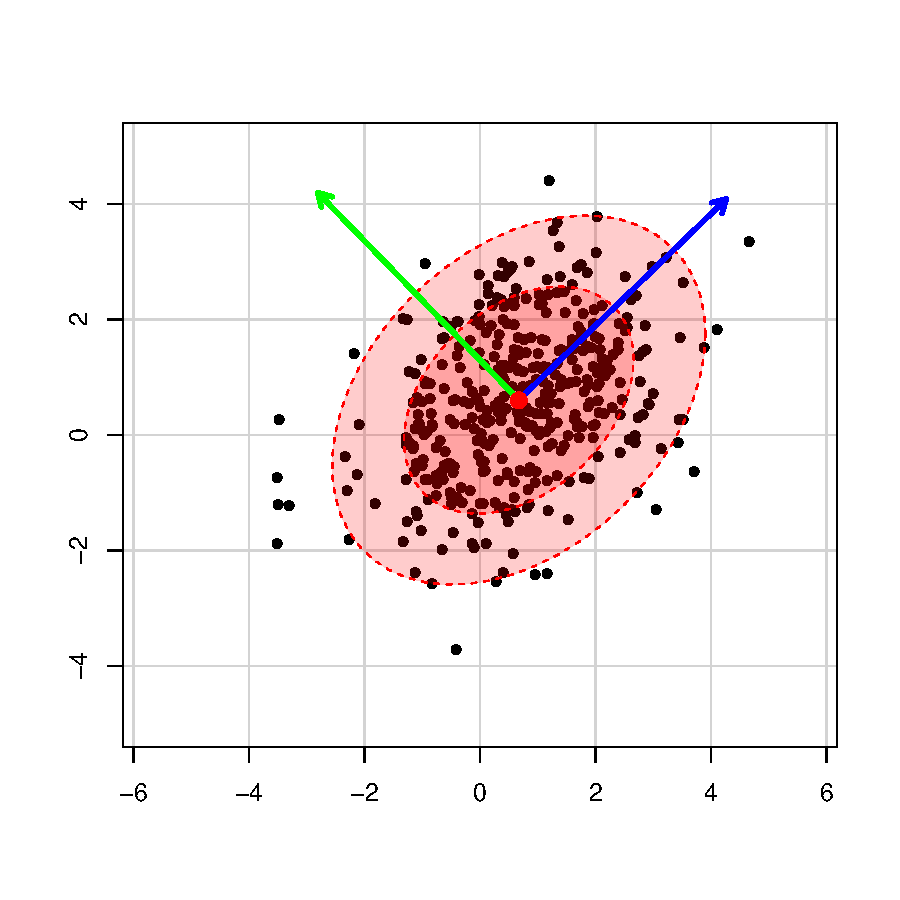
\includegraphics[scale=0.55]{target-distribution-iii.pdf}
\end{center}\vspace*{-1cm}

\begin{triangles}
\item We need to find the origin and semi-axes $\vec{a}_1,\ldots,\vec{a}_n$ of the ellipsoid.
\item Unit vectors $\vec{e}_1,\ldots,\vec{e}_n$ are mapped to semi-axes $\vec{a}_1,\ldots,\vec{a}_n$ of ellipsoid.
\end{triangles}


\foilhead[-1cm]{Variance for a fixed direction}

\textbf{Fact.} Ortogonal projection onto a unit vector $\vec{w}$  is given by scalar product.\vspace*{0.5cm}

\textbf{Question.} What is the direction $\vec{w}$ that maximises the variance for ellipsoid?
\begin{align*}
\VAR(\vec{w}^T \diag(\vec{a})\vec{x})=\VAR\Biggl(\sum_{i=1}^n w_i a_i x_i\Biggr)= \sum_{i=1}^n w_i^2 a_i^2\enspace. 
\end{align*}
The variance is maximised in the direction of the longest ellipse axis $a_1$. \vspace*{0.5cm}


\textbf{Question.}
How is the center of the ellipsoid and mean values connected?
\begin{align*}
\EXP(A\vec{x}+\vec{\mu})=\EXP(A\vec{x})+\EXP(\vec{\mu})= \vec{\mu}\enspace. 
\end{align*}


\foilhead[-1cm]{Principal component analysis}

\begin{triangles}
\item Compute the average value of the observations $\vec{y}_1,\ldots,\vec{y}_m$: 
\begin{align*}
\hat{\vec{\mu}}\gets\frac{\vec{y}_1+\cdots+\vec{y}_m}{m}\enspace.
\end{align*}
\item Centre the data by substituting $\hat{\vec{\mu}}$:
\begin{align*}
\vec{y}_i\gets \vec{y}_i-\hat{\vec{\mu}},\qquad i\in\set{1,\ldots,m}\enspace.
\end{align*}
\item Find the unit direction $\vec{w}_1$ that has \emph{a maximal empirical} variance: 
\begin{align*}
F(\vec{w})=\VAR(\vec{w}^T\vec{y}_1,\ldots,\vec{w}^T\vec{y}_n)=\frac{(\vec{w}^T\vec{y}_1)^2+\cdots+ (\vec{w}^T\vec{y}_m)^2}{m}\enspace.
\end{align*}
\item Find unit directions $\vec{w}_i$ orthogonal to previous directions that maximise the empirical variance of the corresponding the projection onto $\vec{w}_i$.  
\end{triangles}

\foilhead[-1cm]{Covariance matrix and optimisation goal}

We can use matrix algebra to simplify the variance estimate
\begin{align*}
F(\vec{w})&=\frac{1}{m}\cdot\Bigl(\vec{w}^T\vec{y}_1\vec{y}_1^T\vec{w}+\cdots+ \vec{w}^T\vec{y}_m\vec{y}_m^T\vec{w}\Bigr)\\
&=\vec{w}^T\biggl(\frac{\vec{y}_1\vec{y}_1^T+\cdots+\vec{y}_m\vec{y}_m^T}{m}\biggl)\vec{w}
\end{align*}
The $n\times n$ matrix in the middle is known as a \emph{covariance matrix} $\Sigma$.
\vspace*{1cm}

Due to the restriction $\norm{\vec{w}}_2^2=\vec{w}^T\vec{w}=1$, we have to use Lagrange' trick: 
\begin{align*}
F_*(\vec{w})&=\vec{w}^T\Sigma\vec{w}-2\lambda\vec{w}^T\vec{w}
\qquad \Rightarrow\qquad 
\frac{\partial F_*(\vec{w})}{\partial \vec{w}}=2\Sigma\vec{w}- 2\lambda\vec{w}=\vec{0}.
\end{align*}

\foilhead[-1cm]{Principal components as eigenvectors}

The $F_*(\vec{w})$ is maximised only if the direction $\vec{w}$ is an \emph{eigenvector} of $\Sigma$:
\begin{align*}
\Sigma\vec{w}=\lambda\vec{w}\qquad\Rightarrow\qquad \vec{w}^T\Sigma\vec{w}=\vec{w}^T\lambda\vec{w}=\lambda\enspace.
\end{align*}

\textbf{Fact.} If $n\times n$ matrix is symmetric and positively definite then there exists 
$n$ orthogonal eigenvectors $\vec{w}_1,\ldots,\vec{w}_n$ with \emph{eigenvalues} $\lambda_1\geq \ldots\geq\lambda_n>0$. \vspace*{0.5cm}

\textbf{Corollary.} Principal components corresponding to observations $\vec{y}_1,\ldots,\vec{y}_m$ are the eigenvectors of the covariance matrix $\Sigma$. 


\foilhead[-1cm]{Principal component analysis as a rotation}

Reconstruction of the source signal can be viewed as a \emph{translation} followed by a \emph{rotation} to orientate the ellipsoid wrt coordinate axis.

\begin{center}
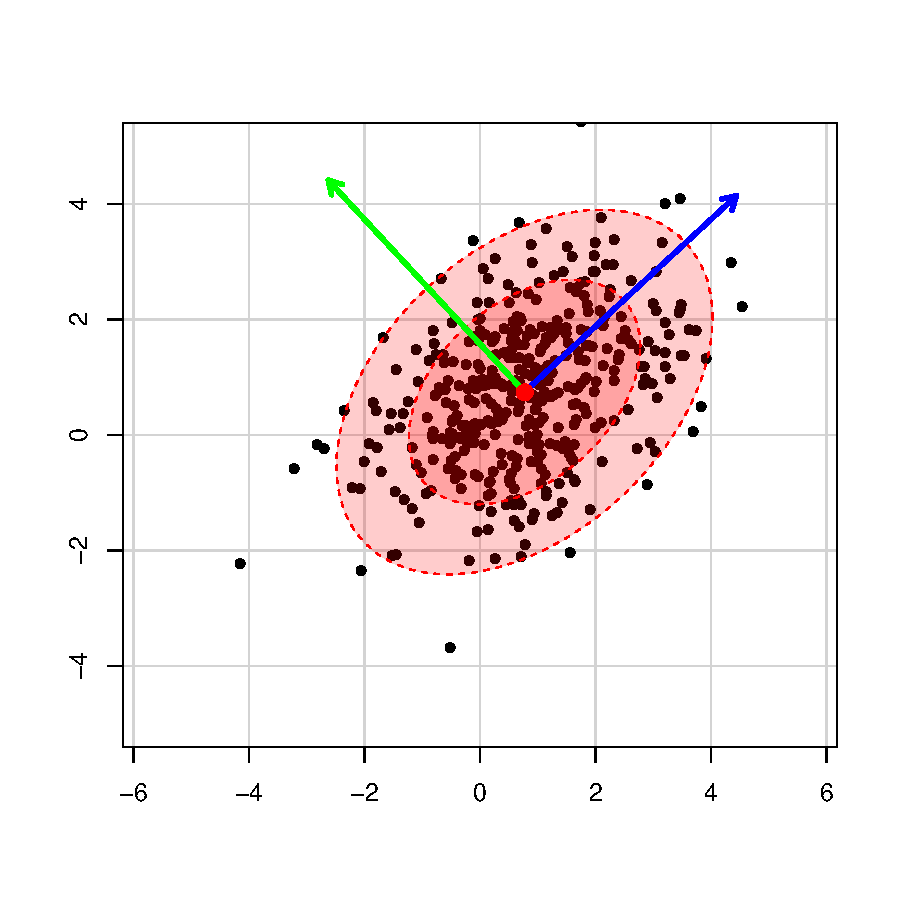
\includegraphics[scale=0.45]{initial-distribution-ii.pdf}
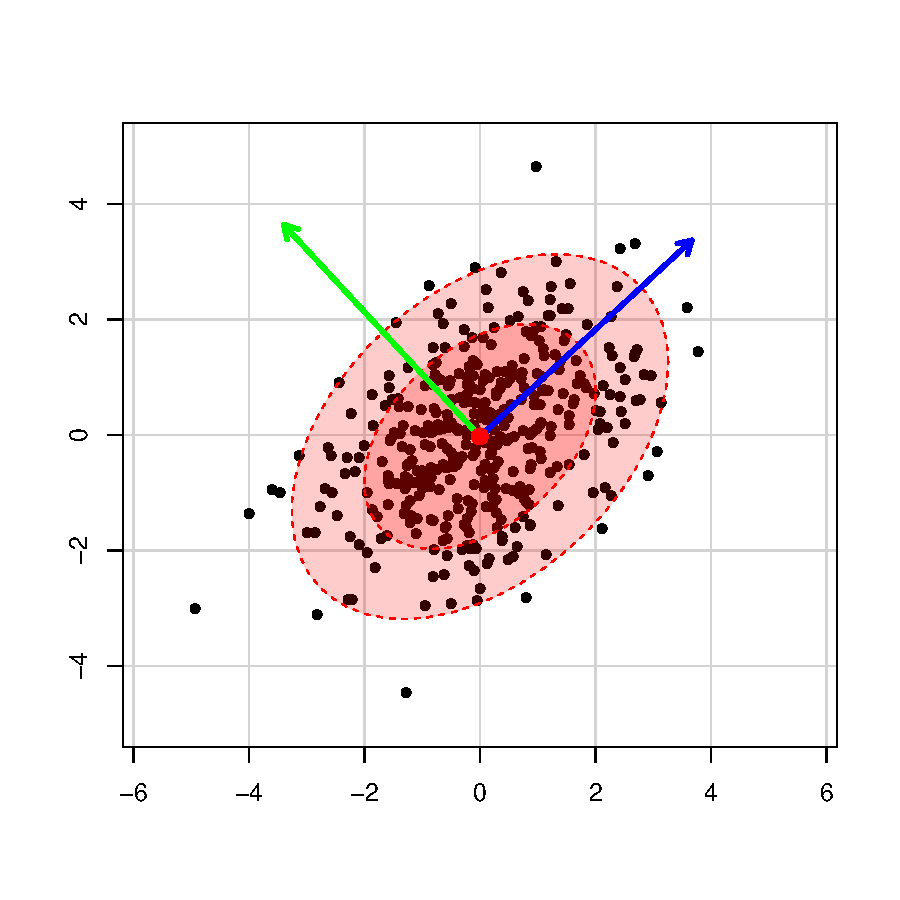
\includegraphics[scale=0.45]{translated-distribution-ii.pdf}
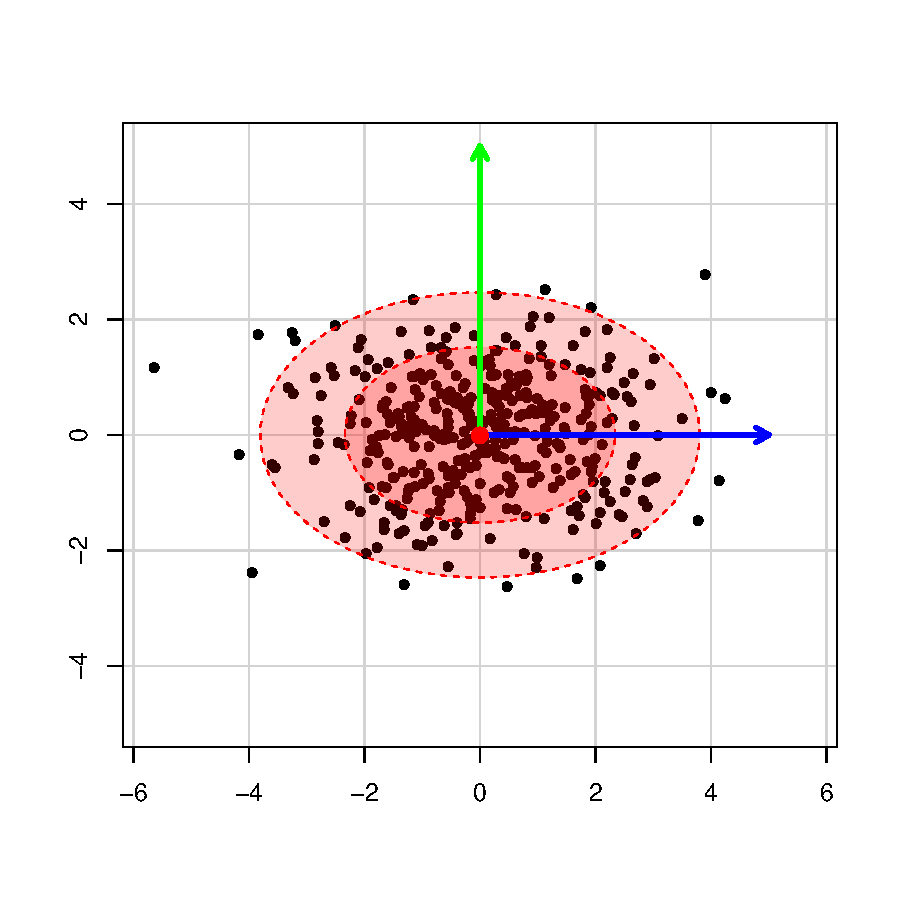
\includegraphics[scale=0.45]{rotated-distribution-ii.pdf}
\end{center}\vspace*{-1cm}

As vectors $\vec{w}_1,\ldots,\vec{w}_n$ are orthogonal, the rotation can be done through computing projections (read scalar products):
\begin{align*}
\hat{\vec{x}}_i= (\vec{w}_1 ||\cdots|| \vec{w}_n)^T (\vec{y}_i-\hat{\vec{\mu}}_0)=W(\vec{y}_i-\hat{\vec{\mu}})\enspace.
\end{align*}  


\foilhead[-1cm]{Maximum likelihood estimate}

The algorithm formulated above was based on \emph{ad hoc} reasoning:
\begin{triangles}
\item Empirical estimates for the mean and variance are not precise!
\end{triangles}\vspace*{1.5cm}

Theoretically correct way to handle the problem is
\begin{triangles}
\item obtain the maximum likelihood estimate on the model parameters,
\item determine the translation and rotation based on the model parameters.
\end{triangles}\vspace*{1.5cm}

What are the model parameters?
\begin{triangles}
\item Parameters of the density formula $\Sigma$ and $\vec{\mu}$.
\item Parameters of the affine transformation $A$ and $\vec{\mu}$.
\end{triangles}

\foilhead[-1cm]{Likelihood function under iid assumption}
If all observations $\vec{y}_1,\ldots,\vec{y}_m$ are independent then\vspace*{-0ex}
\begin{align*}
p[\vec{y}_i,\ldots,\vec{y}_m|\Sigma,\vec{\mu}]
&=\prod_{i=1}^m p[\vec{y}_i|\Sigma,\vec{\mu}]
\end{align*}\vspace*{-4ex}\\
where\vspace*{-0ex}
\begin{align*}
p[\vec{y}_i|\Sigma,\vec{\mu}]
&=\frac{1}{(2\pi)^{n/2}}\cdot\frac{1}{\sqrt{\det(\Sigma)}}\cdot
\exp{-\frac{(\vec{y}_i-\vec{\mu})^T \Sigma^{-1}(\vec{y}_i-\vec{\mu})}{2}}\enspace
\end{align*}\vspace*{-0ex}\\
The \emph{log-likelihood} of the data $\ln p[\vec{y}_i,\ldots,\vec{y}_m|\Sigma,\vec{\mu}]$ can be expressed \vspace*{-0ex}
\begin{align*}
\LLL(\Sigma,\vec{\mu})=const +\frac{m}{2}\cdot \ln\det(\Sigma^{-1}) 
-\sum_{i=1}^m\frac{(\vec{y}_i-\vec{\mu})^T \Sigma^{-1}(\vec{y}_i-\vec{\mu})}{2}
\end{align*}
Now we have to find the arrangement $(\Sigma,\vec{\mu})$ that maximises $\LLL(\Sigma,\vec{\mu})$.\lastline
 
\foilhead[-1cm]{Gradients of the log-likelihood function}

Gradient with respect to the shift $\vec{\mu}$: 
\begin{align*}
\frac{\partial\LLL}{\partial\vec{\mu}}= -\sum_{i=1}^m\frac{\partial}{\partial\vec{\mu}}\frac{(\vec{y}_i-\vec{\mu})^T \Sigma^{-1}(\vec{y}_i-\vec{\mu})}{2}
=-\sum_{i=1}^m\frac{\Sigma^{-1}(\vec{y}_i-\vec{\mu})}{2}\cdot(-1)
\end{align*}
Gradient with respect to the inverse matrix $\Sigma^{-1}$: 
\begin{align*}
\frac{\partial\LLL}{\partial(\Sigma^{-1})}&=\frac{m}{2}\cdot \frac{\partial}{\partial(\Sigma^{-1})} \ln\det(\Sigma^{-1}) -\sum_{i=1}^m\frac{\partial}{\partial(\Sigma^{-1})}\frac{(\vec{y}_i-\vec{\mu})^T \Sigma^{-1}(\vec{y}_i-\vec{\mu})}{2}\\
&=\frac{m}{2}\cdot\Sigma^{T} -\sum_{i=1}^m\frac{(\vec{y}_i-\vec{\mu})^T (\vec{y}_i-\vec{\mu})}{2}
\end{align*}
As $\Sigma$ is symmetric and $\Sigma^{-1}$ exists we can derive closed form solutions.

\foilhead[-1cm]{Maximum likelihood estimates for parameters}

The shift must be the mean of all observations
\begin{align*}
\vec{\mu}=\frac{1}{m}\cdot \sum_{i=1}^m\vec{y}_i\enspace.
\end{align*} 
The covariance matrix 
\begin{align*}
\Sigma=\frac{1}{m}\cdot\sum_{i=1}^m(\vec{y}_i-\vec{\mu})^T (\vec{y}_i-\vec{\mu})
\end{align*}

\textbf{Correctness of PCA.}
As ML estimates are exactly the same  we used in principal component analysis, the method is theoretically justified!\lastline


\middlefoil{Principal component analysis\vspace*{1ex}\\
 Alternative formalisations}

\foilhead[-1cm]{Dimensionality reduction}

What if the actual data $\vec{x}_1,\ldots,\vec{x}_m$ lies in a lower-dimensional plane and the observation  $\vec{y}_1,\ldots,\vec{y}_m$ are obtained by random shifts?   



\begin{center}
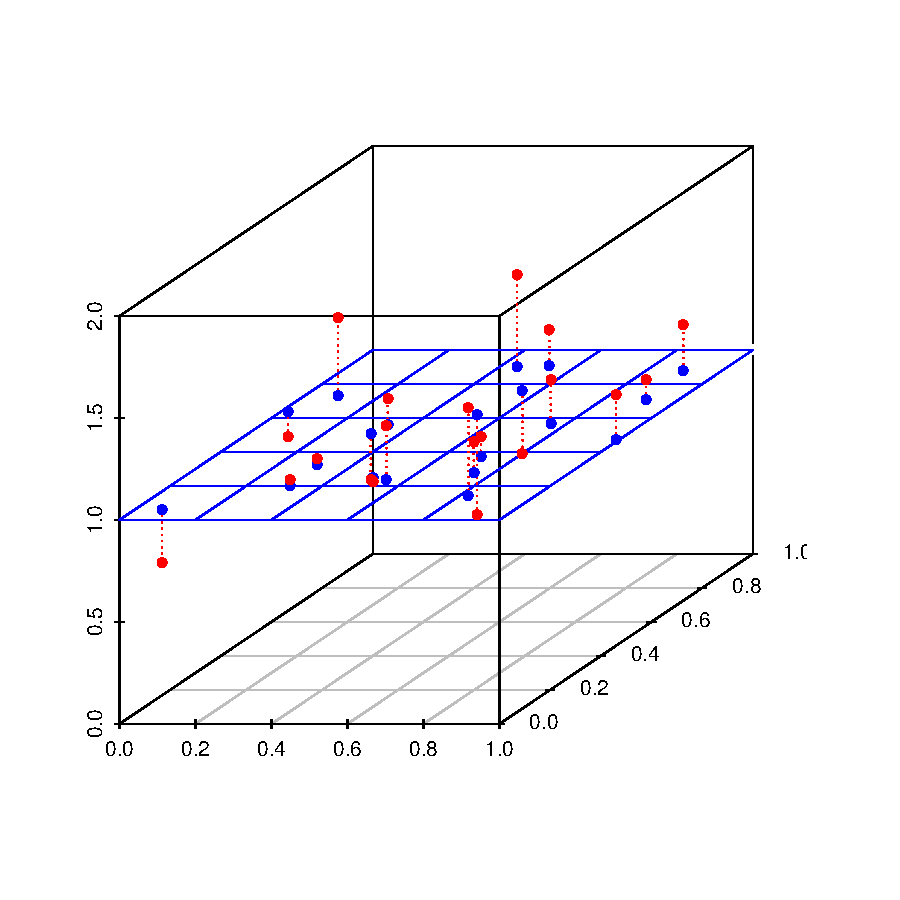
\includegraphics[scale=0.55]{low-dimensional-data-i.pdf}
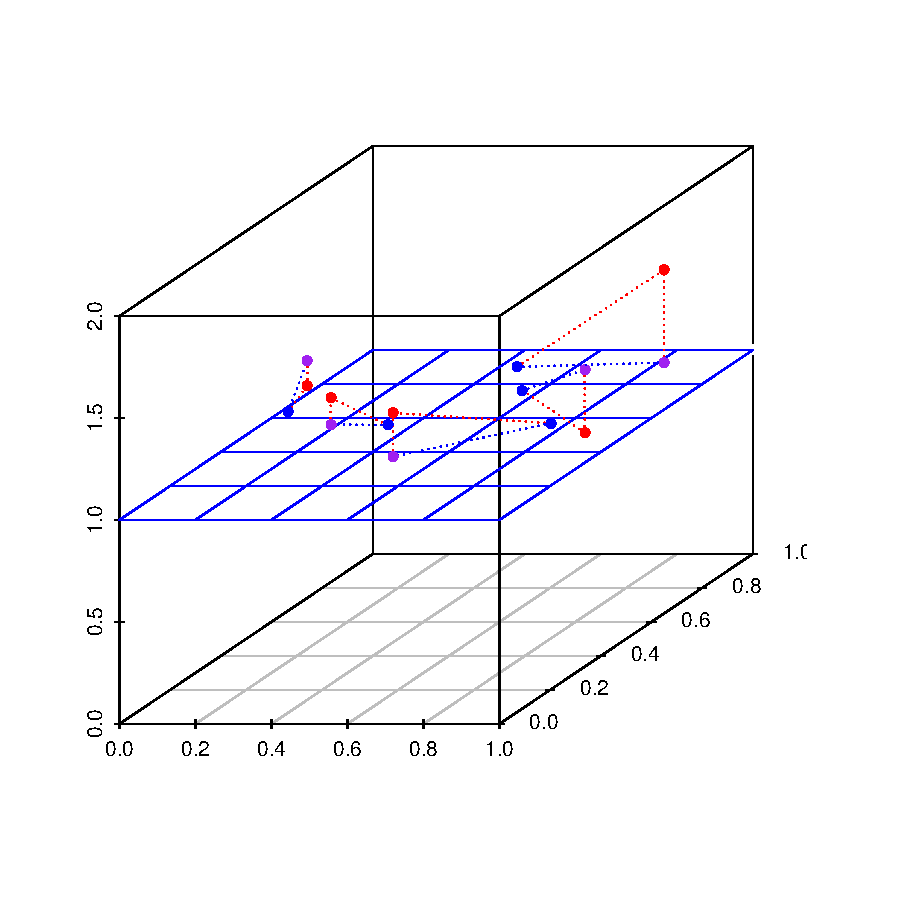
\includegraphics[scale=0.55]{low-dimensional-data-ii.pdf}
\end{center}\vspace*{-1cm}

The shifts can be either orthogonal to the plane or just random. The first model is easier to analyse while the second is more plausible. 


\foilhead[-1cm]{Maximum likelihood estimate}

Let $\HHH$ be the plane. Assume that the random shifts $\varepsilon_i$ are orthogonal to the plane and have a normal distribution $\NNN(0,\sigma I)$. Then 
\begin{align*}
p[\vec{y}_i|\HHH,\sigma]=const\cdot\exp{-\frac{d_i^2}{2\sigma^2}}
\end{align*}
where $d_i$ is the distance between the plane $\HHH$ and the point $\vec{y}_i$. Thus
\begin{align*}
p[\vec{y}_1,\ldots,\vec{y}_m|\HHH,\sigma]=const\cdot\exp{-\sum_{i=1}^m\frac{d_i^2}{2\sigma^2}}
\end{align*}
and the maximum likelihood estimate of the plane minimises sum of the distance squares. Corresponding estimates of $\vec{x}_1,\ldots,\vec{x}_m$ are projections of $\vec{y}_1,\ldots,\vec{y}_m$ to the plane $\HHH$.\lastline 

\foilhead[-1cm]{Another characterisation of PCA}

\textbf{Fact.} If the data is centred then PCA chooses the direction $\vec{w}_1$ such that
the sum of squares of the projections $\vec{w}_1^T \vec{y}_i$ is maximal.\vspace*{-1cm}

\begin{center}
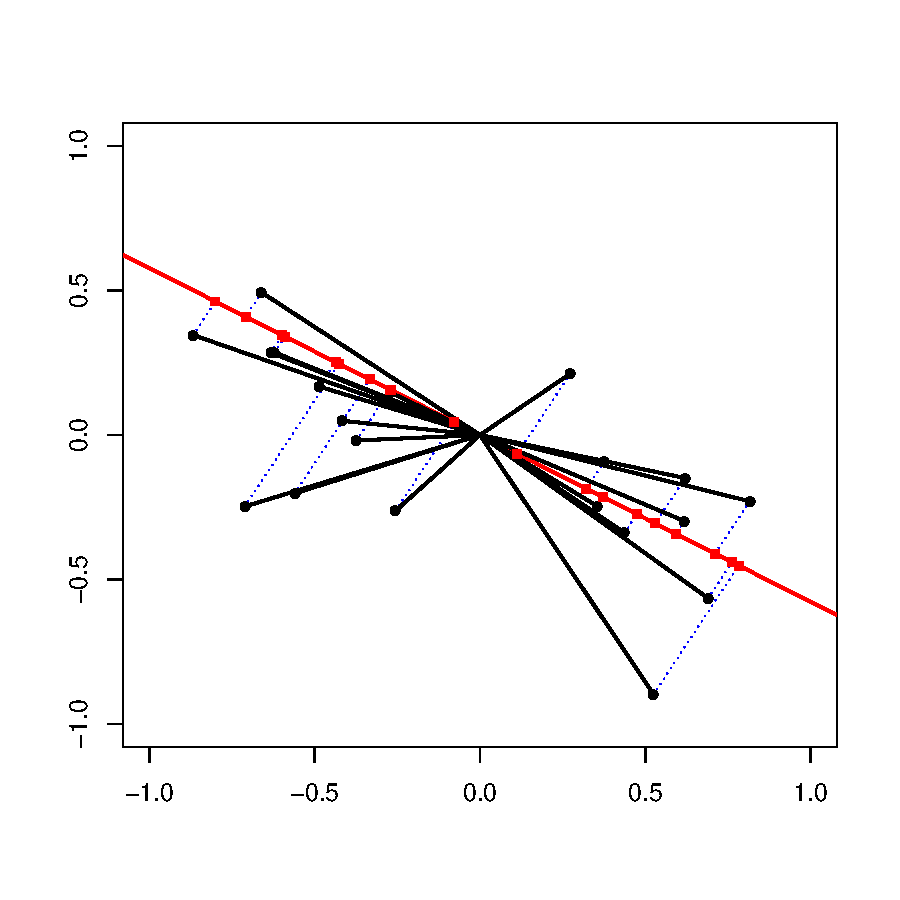
\includegraphics[scale=0.65]{orthogonal-projection.pdf}
\end{center}\vspace*{-1cm}


\textbf{Corollary.} PCA chooses directions $\vec{w}_1,\ldots,\vec{w}_n$ such that the sum of distance squares from the hyperplane formed by $\vec{w}_1,\ldots,\vec{w}_k$ is minimal. 

\foilhead[-1cm]{PCA as a dimensionality reduction tool}

\textbf{Corollary.} PCA rotates the data such way that first $k$ coordinates of the rotated data correspond to maximum likelihood reconstructions of original vectors corrupted with white Gaussian noise $\NNN(0,\sigma I)$.  


\begin{center}
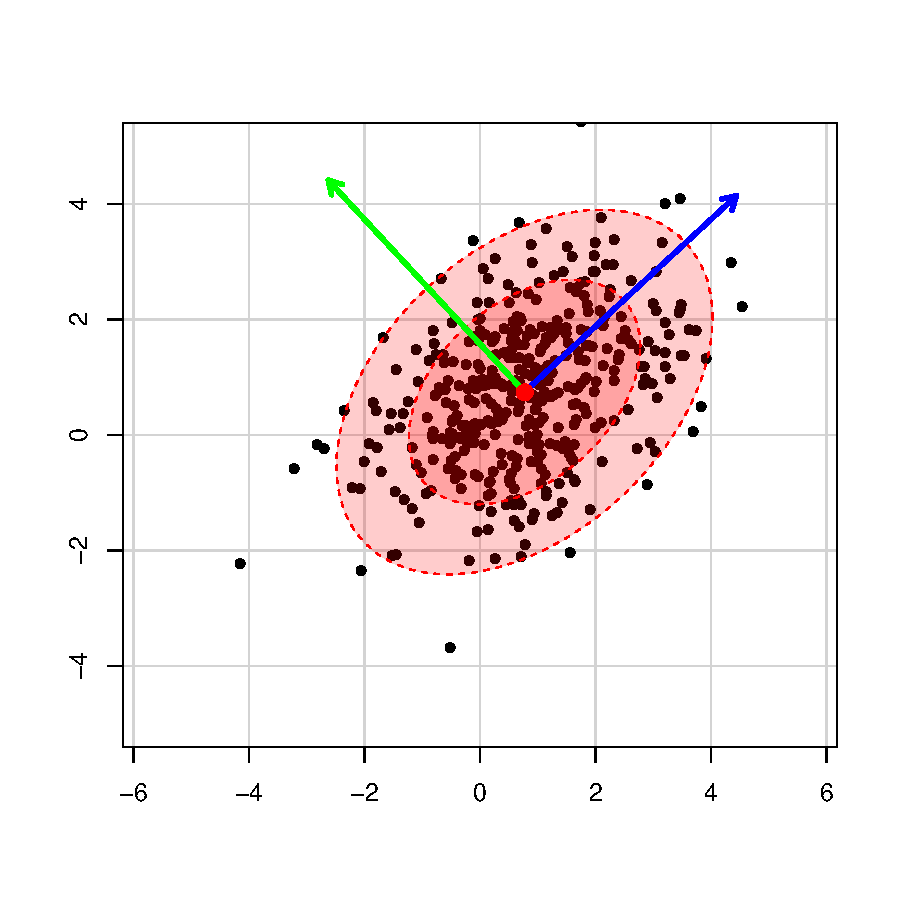
\includegraphics[scale=0.45]{initial-distribution-ii.pdf}
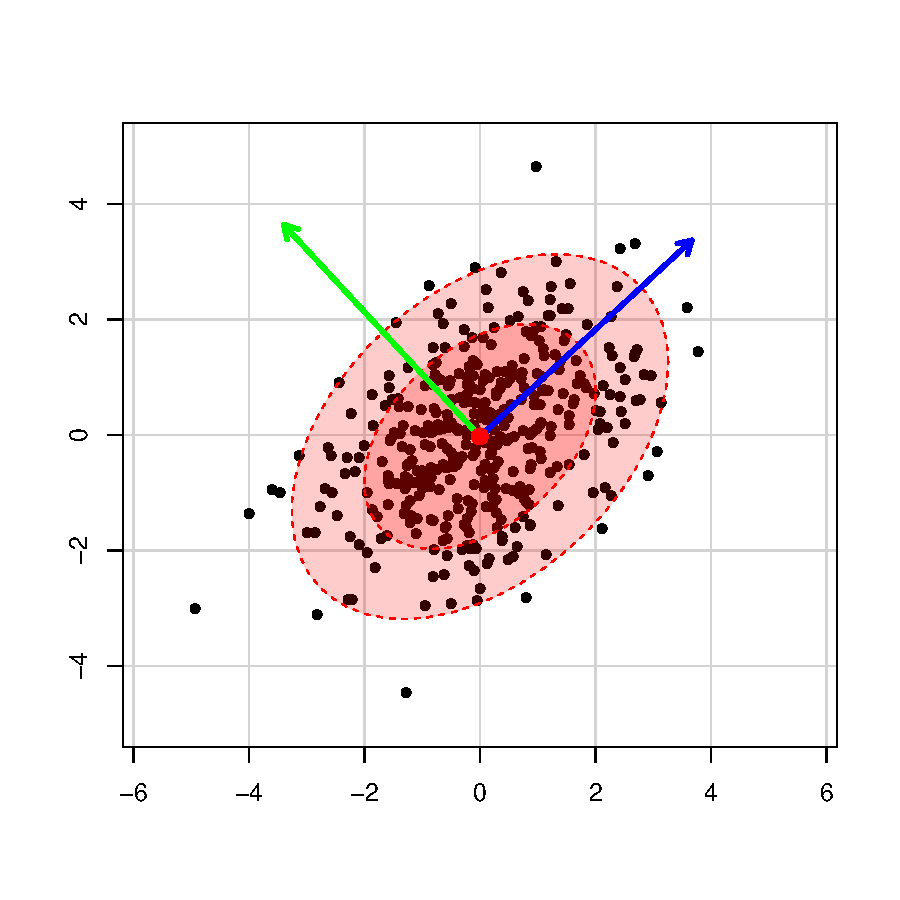
\includegraphics[scale=0.45]{translated-distribution-ii.pdf}
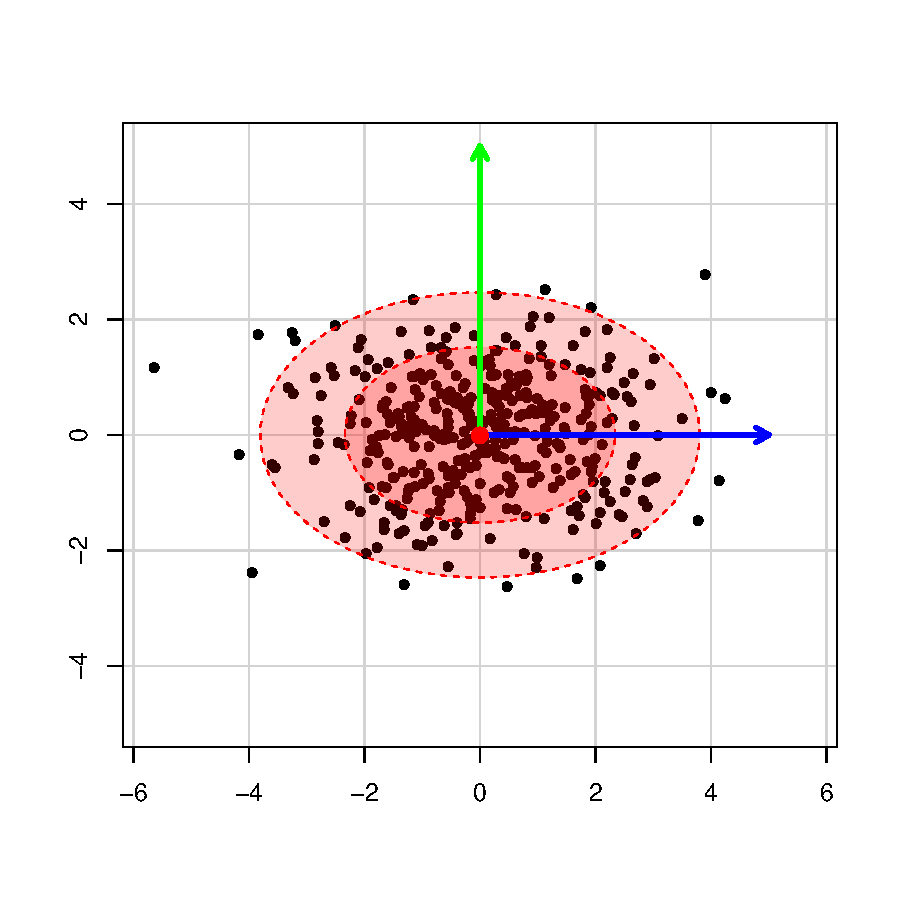
\includegraphics[scale=0.45]{rotated-distribution-ii.pdf}
\end{center}\vspace*{-1cm}

Alternatively, we can view the last components of the source signal $\vec{x}$ as the uninformative noise. The overall noise component should be small.\lastline

\foilhead[-1cm]{Going beyond PCA}

Weighted Principal Component Analysis:
\begin{triangles}
\item Sometimes data contains potential outliers.
\item Sometimes we can assign reliability scores to the data points. 
\end{triangles}\vspace*{1.0cm}

Principal curves and manifolds
\begin{triangles}
\item The original data might be on a low dimensional manifold. 
\item The observed data is corrupted by additive white gaussian noise. 
\item The task is to reconstruct the manifold and ML estimate for the data. 
\end{triangles}\vspace*{1.0cm}


Independent Component Analysis 
\begin{triangles}
\item What if the source components are non-gaussian? 
\item Then the reconstruction is possible up to scaling!
\end{triangles} 


\foilhead[-3cm]{Principal curves and manifolds}

\begin{center}
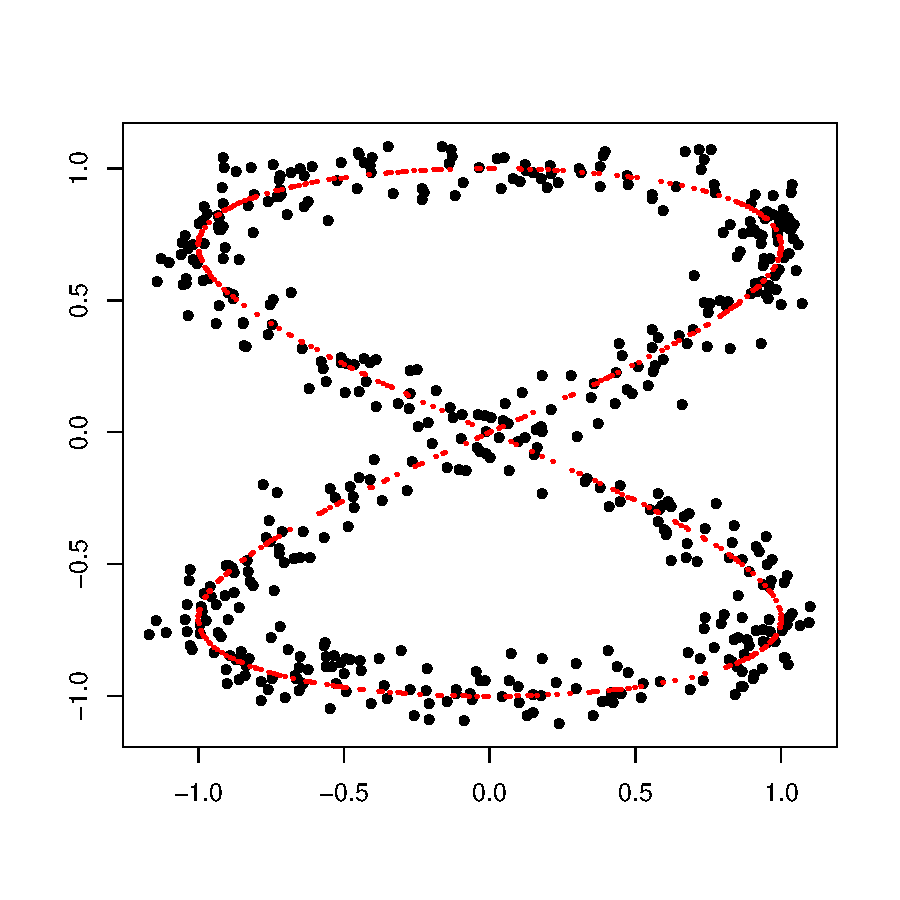
\includegraphics[scale=0.75]{principal-curve.pdf}
\end{center}\vspace*{-1cm}

Reconstruction of the underlying curve is much more difficult.
\begin{triangles}
\item We must fix a curve parametrisation 
\item The task is different form regression since we have only outputs.
\end{triangles} 
 


\foilhead[-1cm]{Independent Component Analysis}

Assume that the components of the source data $\vec{x}_1,\ldots,\vec{x}_m$ are independent  
but an unknown affine transformation  $\vec{y}=A\vec{x}+\vec{\mu}$ disturbs observations. 
\begin{center}
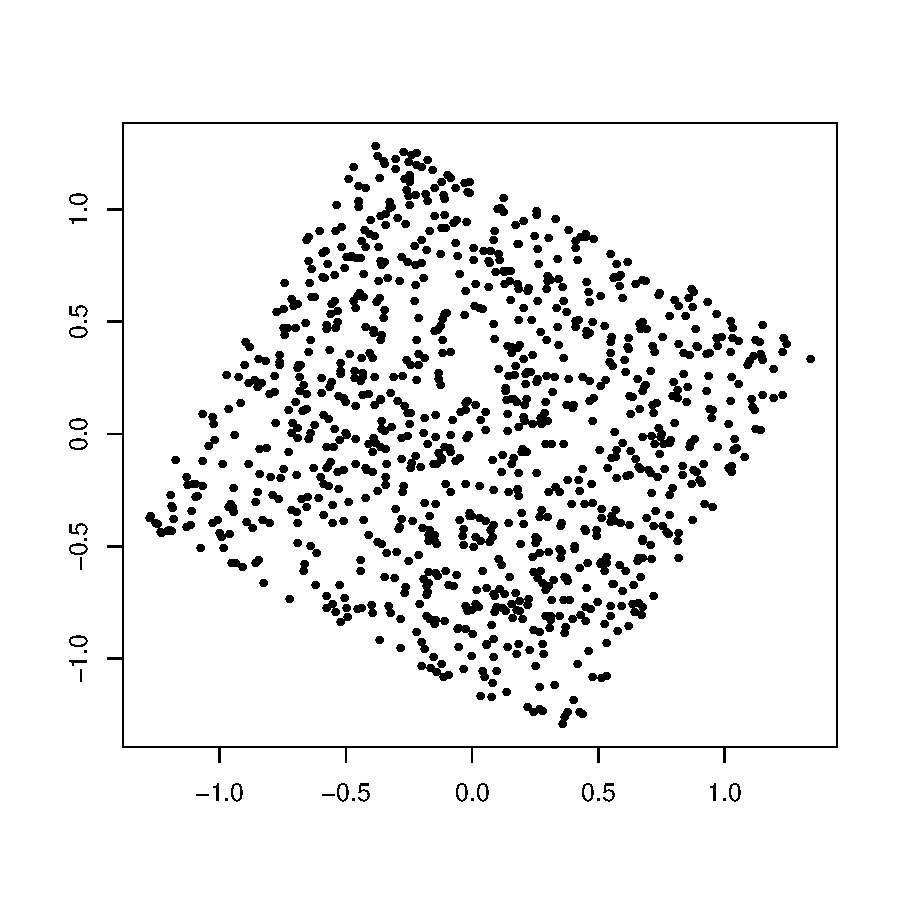
\includegraphics[scale=0.45]{ica-i.pdf}
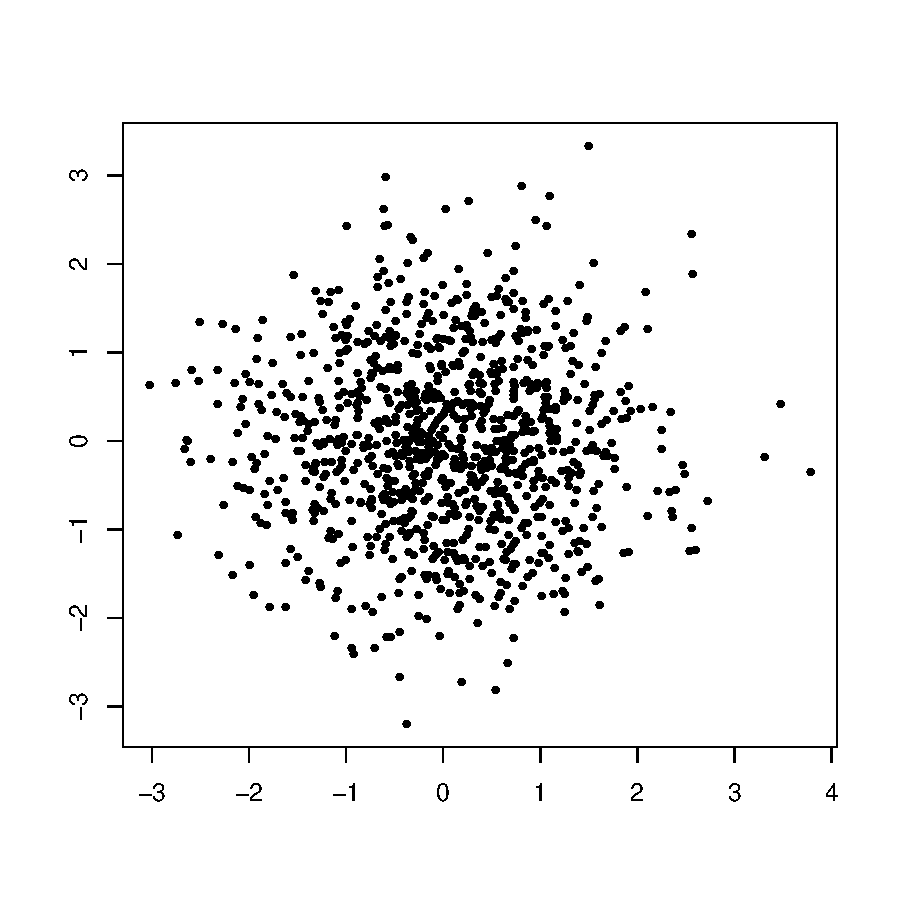
\includegraphics[scale=0.45]{ica-ii.pdf}
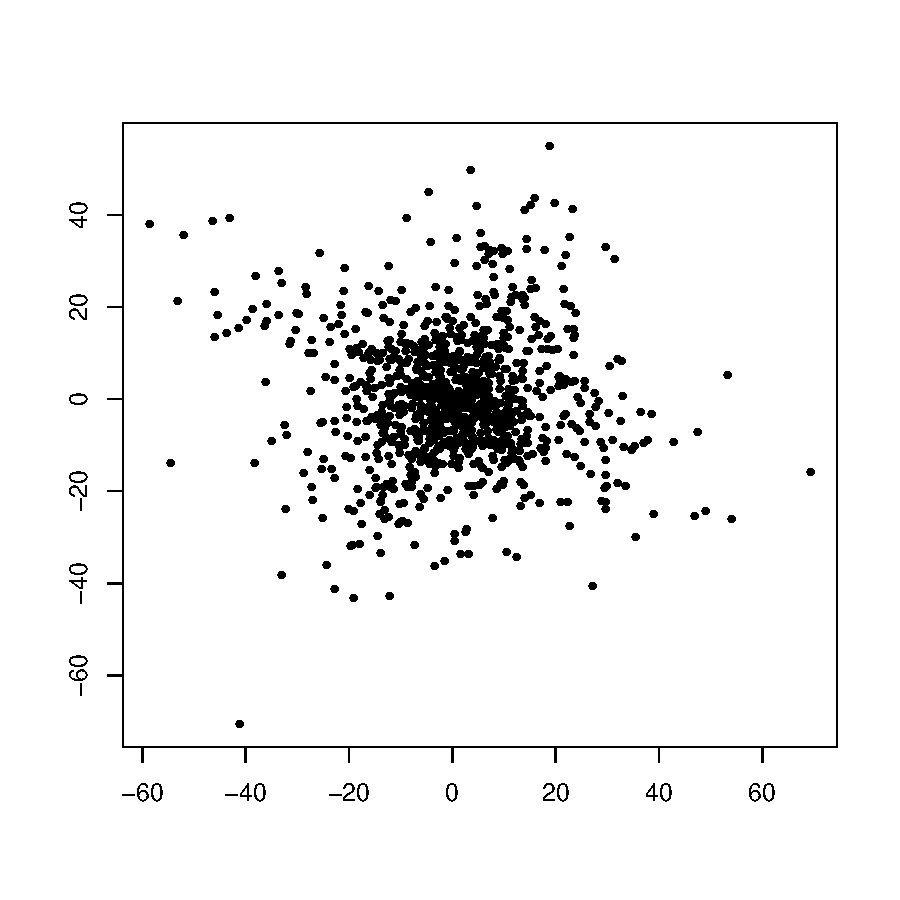
\includegraphics[scale=0.45]{ica-iii.pdf}
\end{center}\vspace*{-1cm}

It is possible to recover the translation and rotation only if independent components are sufficiently different form the normal distribution.  


\end{document}

\foilhead[-1cm]{How to choose a model?}

Assume that there are $k$ models $\MMM_1,\ldots, \MMM_k$ that could
potentially explain the data $\DDD=\set{(\vec{x_1},y_1),\ldots,
  (\vec{x}_n, y_n)}$. What model should we choose?

\begin{triangles}
  \item Bayes formula leads to posterior probabilities
    \begin{align*}
      \pr{\MMM_i|\DDD}=\frac{\pr{(\vec{x}_1,y_1),\ldots,(\vec{x}_n,
          y_n)|\MMM_i}\pr{\MMM_i}}
        {\pr{(\vec{x}_1,y_1),\ldots,(\vec{x}_n, y_n)}}
    \end{align*}
  \item If I have to choose only one model, then I should choose the
    one with the highert posterior probability.
  \item My choice depends on prior probabilities
    $\pr{\MMM_1},\ldots,\pr{\MMM_k}$.
\end{triangles}

\foilhead[0cm]{Illustrative example}

\illustration[height=9.5cm]{discrete-coinflipping-model-10} 
\vspace*{-1cm}

Consider a series of coin flips $\vec{x}=(1,0,1,0,1,0,1,0)$ and potential bias parameter values $\alpha=\set{0.0, 0.1,\ldots, 0.9,1.0}$. Then we can use the Bayes formula and find the $\alpha$ value with the highest probability. 



\foilhead[0cm]{Illustrative example}

\illustration[height=9.5cm]{discrete-coinflipping-model-biased-10} 
\vspace*{-1cm}

However, note that a different prior can lead to completely different results. 


\foilhead[-1cm]{Maximum likelihood principle}

If I have no background information to prefer one model to another then 
\begin{align*}
  \pr{\MMM_i}=const
\end{align*}
and thus 
\begin{align*}
  \pr{\MMM_i|\DDD} = const\cdot \pr{(\vec{x}_1,y_1),\ldots,(\vec{x}_n,
          y_n)|\MMM_i}
\end{align*}
As a result I should choose a model that maximises \emph{likelihood}
\begin{align*}
  \pr{(\vec{x}_1,y_1),\ldots,(\vec{x}_n, y_n)|\MMM_i}
\end{align*}
The same principle is also applicable if the number of models is infinite.

\foilhead[-0cm]{Illustrative example continued ...}

\illustration[height=10cm]{discrete-coinflipping-model-10b}
\vspace*{-0.5cm}

For the observation vector $\vec{x}=(1,0,1,0,1,0,1,0)$, the assumption that  $\alpha\in\set{0.0, 0.1,\ldots, 0.9, 1.0}$ provides a rather coarse choice of models ...

\foilhead[-0cm]{Illustrative example continued ...}

\illustration[height=10cm]{discrete-coinflipping-model-100b}
\vspace*{-0.5cm}


The assumption that $\alpha\in\set{0.00, 0.01,\ldots, 0.99, 1.00}$ is better ...

\foilhead[-0cm]{Illustrative example continued ...}


\illustration[height=10cm]{discrete-coinflipping-model-1000b}
\vspace*{-0.5cm}

The assumption that $\alpha\in\set{0.000, 0.001,\ldots, 0.999, 1.000}$ is even better ...


\foilhead[-1cm]{ML estimate for coin-flipping}

\textbf{Set of models.} Let model $\MMM_\alpha$ denote settings where
$x_1,\ldots,x_n$ are drawn from Bernoulli distribution (independent coin-tosses):
\begin{align*}
  \pr{x_1,\ldots,x_n|\MMM_\alpha}=\alpha^k(1-\alpha)^{n-k}
\end{align*}
where the $k$ is the number of ones in the series $x_1,\ldots,x_k$.
\bigskip

\textbf{Maximisation task.} To solve
$F(\alpha)=\alpha^k(1-\alpha)^{n-k}\to \max$ we have to solve
\begin{align*}
  \frac{\partial F}{\partial \alpha}=\alpha^{k-1}(1&-\alpha)^{n-k-1}(k(1-\alpha)-(n-k)\alpha)=0\\
\end{align*}
From which we get $\alpha=k/n$.



\foilhead[-1cm]{ML and linear regression}

\textbf{Set of models.} Let model $\MMM_{a,b}$ denote settings where
$x_1,\ldots,x_n$ are drawn from the normal distribution $\NNN(0,1)$
and $y_1,\ldots,y_n$ are computed as
\begin{align*}
  y_i=ax_i+b+\varepsilon_i,\qquad \varepsilon_i\sim\NNN(0,\sigma^2)
\end{align*}
Now note that 
\begin{align*}
  p[\DDD|a,b]&=\prod_{i=1}^n\frac{1}{\sqrt{2\pi}}\exp{-\frac{x_i}{2}}\cdot \frac{1}{\sqrt{2\pi}
    \sigma}\cdot\exp{-\frac{(y_i-ax_i-b)}{2\sigma^2}}\\
   &const\cdot\underbrace{\exp{-\frac{(y_i-ax_i-b)^2}{2\sigma^2}}}_{F(a,b)}
\end{align*}

\foilhead[-1cm]{Illustrative example}

\begin{center}
\includegraphics[width=8cm, trim = 3cm 1cm 2cm 2cm, clip]{linear-regression-model-1}\hspace*{0cm}
\includegraphics[width=8cm, trim = 3cm 1cm 2cm 2cm, clip]{linear-regression-model-2}
\end{center}
\vspace*{0.5cm}

For instance, models with parameters $y=x$ and $y=-x$ generate the following probability distribution when $\sigma=0.5$. 
\vspace*{-0.5cm}



\foilhead[-1cm]{Further analysis}

To maximise 

\begin{align*}
 F(a,b) =\exp{-\frac{(y_i-ax_i-b)^2}{2\sigma^2}}
\end{align*}
 we can solve the minimisation task 
\begin{align*}
  \frac{(y_i-ax_i-b)^2}{2\sigma^2}\to\min
\end{align*}
with respect to $a$ and $b$. We have obtained justification for the
standard formalisation of linear regression.

\foilhead[-2cm]{ML and neural networks} 

\textbf{Set of models.} The set of models is fixed with a the topology
of neural network and weight vector $\vec{w}$. Let
$f_{\vec{w}}(\vec{x})$ be the models response to the input
$\vec{x}$. As before, we can define
\begin{align*}
  y_i=f_{\vec{w}}(\vec{x}_i)+\varepsilon_i,\qquad
  \varepsilon_i\sim\NNN(0,\sigma^2)
\end{align*}
Now note that 
\begin{align*}
  p[\DDD|\vec{w}]&=const\cdot\prod_{i=1}^n\exp{-\frac{(y_i-f_{\vec{w}}(\vec{x}_i))^2}{2\sigma^2}}
\end{align*}
and thus we must solve the following optimisation task 
\begin{align*}
 \sum_{i=1}^n (y_i-f_{\vec{w}}(\vec{x}_i))^2\to \min.
\end{align*}
\enlargethispage{2cm}

\foilhead[-1cm]{Illustrative example}


\begin{center}
\includegraphics[width=8cm, trim = 3cm 1cm 2cm 2cm, clip]{cubic-regression-model}\hspace*{0cm}
\includegraphics[width=8cm, trim = 3cm 1cm 2cm 2cm, clip]{sinus-regression-model}
\end{center}
\vspace*{0.5cm}


\foilhead[-1cm]{Predictions and sanity checks}

Assume that ML estimate is precise enough then residues
\begin{align*}
  \Delta_i=y_i-f_{\vec{w}}(\vec{x}_i)
\end{align*}
must be roughly distributed according to $\NNN(0,\sigma)$ and we can
estimate
\begin{align*}
  \sigma=\sqrt{\frac{1}{n}\sum_{i=1}^n{(y_i-f_{\vec{w}}(\vec{x}_i))^2}}\enspace.
\end{align*}
Now we can compute $95\%$ confidence intervals for predictions:
\begin{triangles}
  \item Around 95\% of predictions should be in the confidence interval
  \item Residues should have normal distribution.
\end{triangles}
 
\foilhead[-1.5cm]{Beyond Gaussian noise}

Sometimes we have too many outliers in the data. Such points will have
high leverage since the distribution has light tails. There are two alternatives
\begin{triangles}
  \item Use heavy-tail error distribution instead of normal distribution
  \item Model outlier points separately.
\end{triangles}
\vskip 1cm


Usually the problem is solved by using centred Laplace distribution
\begin{align*}
  p[\varepsilon|\beta]=\frac{1}{2\beta}\cdot \exp{-\frac{\abs{\varepsilon}}{\beta}}
\end{align*}
As a result, we get a minimisation task
\begin{align*}
  \sum_{i=1}^n\abs{y_i-f_{\vec{w}}(x_i)}\to \min\enspace.
\end{align*}

\foilhead[-1cm]{Quick hack to implement second approach}

To implement the second strategy, we have to find outlier points. For
that, we can cycle the following algorithm till convergence:\\


\begin{triangles}
  \item Train a model on normal data points.
  \item Estimate standard deviation of the noise $\sigma$.
  \item Use $\sigma$ to compute $95\%$ confidence intervals for each data point.
  \item Label all points outside the confidence interval as outliers.    
\end{triangles}
\vspace*{1cm}

More advanced techniques require mixture modelling and EM-algorithm.

\foilhead[-1cm]{Illustrative example}


\begin{center}
\includegraphics[width=10cm]{fit-with-outliers}\hspace*{0cm}
\includegraphics[width=10cm]{fit-without-outliers}
\end{center}
\vspace*{0.5cm}

Model fits the data much better if we remove most obvious outliers.


\foilhead[-1cm]{Maximum a posteriori principle}

Sometimes, we have extra background knowledge that makes some models
more likely than the others:
\begin{align*}
  \pr{\MMM_i}\neq const
\end{align*}
Then the model with largest likelihood is suboptimal choice and we
should take a model with highest posterior probability
\begin{align*}
  \pr{\MMM_i|\DDD}\to\max\enspace.
\end{align*}
This method is known as \emph{maximum a posteriori principle}.\\

In most cases, MAP estimates are defined so that they are
\emph{numerically and statistically more stable} than ML estimates.

\foilhead[-1cm]{MAP and linear regression}

Let $f(\vec{x})=w_1x_1+\ldots+w_kx_k+w_0$. Then the restriction 
\begin{align*}
  \norm{\vec{w}}_1=\abs{w_0}+\cdots+\abs{w_k}\leq c
\end{align*}
guarantees that $\abs{f(\vec{x})}\leq c$ in the range
$x_i\in[-1,1]$. 

Hence, if I have background information that $f$ is
bounded in this range then I should assign prior
\begin{align*}
  p(\vec{w})=
  \begin{cases}
    const &\text{if }\norm{\vec{w}}_1\leq c\enspace,\\
    0 &\text{if } \norm{\vec{w}}_1>c\enspace.
  \end{cases}
\end{align*}

\foilhead[-3cm]{Further analysis}

\begin{align*}
  p[\vec{w}|\DDD]=
  \begin{cases}
    const\cdot \exp{-\sum_{i=1}^n(y_i-f_{\vec{w}}(\vec{x}_i))^2} &\text{if } \norm{\vec{w}}\leq c\enspace,\\
    0  &\text{if } \norm{\vec{w}}> c\enspace,
  \end{cases}
\end{align*}
Hence, we must solve the following minimisation trick
\begin{align*}
  \sum_{i=1}^n(y_i-f_{\vec{w}}(\vec{x}_i))^2\to \min\qquad  \text{s.t. } \norm{\vec{w}}_1\leq c
\end{align*}
Lagrange trick yields a non-constrained optimisation task\vspace*{-0.5cm}
\begin{align*}
  \sum_{i=1}^n(y_i-f_{\vec{w}}(\vec{x}_i))^2+\lambda \norm{\vec{w}}_1\enspace.
\end{align*}\vspace*{-1.5cm}

This is known as \emph{lasso} regression method
\enlargethispage{1cm}


\foilhead[-1cm]{MAP and ridge regression}

Let $f(\vec{x})=w_1x_1+\ldots+w_kx_k+w_0$. Then the restriction 
\begin{align*}
  \norm{\vec{w}}_2^2=w_0^2+\cdots+w_k^2\leq c
\end{align*}
guarantees that $\abs{f(\vec{x})}\leq c$ in the range
$x_1^2+\cdots+x_k^2\leq 1$. Hence, if I have background information
that $f$ is bounded in this range then
\begin{align*}
  p(\vec{w})=
  \begin{cases}
    const &\text{if }\norm{\vec{w}}_2^2\leq c\enspace,\\
    0 &\text{if } \norm{\vec{w}}_2^2>c\enspace.
  \end{cases}
\end{align*}
as a result we get
\begin{align*}
  \sum_{i=1}^n(y_i-f_{\vec{w}}(\vec{x}_i))^2+\lambda \norm{\vec{w}}_2^2\enspace.
\end{align*}
\enlargethispage{2cm}

\foilhead[-1cm]{Going backwards}

Penalised mean square errors can be traced back to a different prior 

\begin{align*}
 p[\MMM|\DDD]&=const\cdot\exp{-\sum_{i=1}^n(y_i-f_{\vec{w}}(\vec{x}_i))^2-\lambda \norm{\vec{w}}_2^2}\\  
 p[\MMM|\DDD] &=const\cdot p[\DDD|\MMM]\cdot\underbrace{\exp{-\lambda \norm{\vec{w}}_2^2}}_{p[\MMM]}
\end{align*}
As the last term corresponds to centred multivariate normal
distribution, we know that ridge regression assigns normal prior to
$\vec{w}$.
\begin{triangles}
  \item Prior is invariant under coordinate rotations 
  \item Larger $\lambda$ shrinks the distribution towards zero.
\end{triangles}
\end{document}
 
\foilhead[-1cm]{ML and Gaussian classifier}

Assume that data points come from two distributions
\begin{align*}
  \vec{x}_i&\sim\NNN(\vec{\mu}_0,\Sigma_0)\qquad\text{if } y_i=0\\ 
  \vec{x}_i&\sim\NNN(\vec{\mu}_1,\Sigma_1)\qquad\text{if } y_i=1
\end{align*}
As a result 
\begin{align*}
  p[\DDD|\MMM]&=const\cdot
  \prod_{i=1}^n\abs{\Sigma_{y_i}}^{-1/2}\exp{-\frac{1}{2}(\vec{x}_i-\vec{\mu}_{y_i})^t\Sigma_{y_i}(\vec{x}_i-\vec{\mu}_{y_i})}\\
&= const\cdot F_0(\vec{\mu}_0,\Sigma_0)\cdot F_1(\vec{\mu}_0,\Sigma_0)
\end{align*}
where
\begin{align*}
  F_j(\vec{\mu}_j,\Sigma_j)= \prod_{j:y_i=j}\abs{\Sigma_{j}}^{-1/2}\exp{-\frac{1}{2}(\vec{x}_i-\vec{\mu}_{j})^t\Sigma_{i}(\vec{x}_i-\vec{\mu}_{j})}
\end{align*}
Fortunately, we can optimise $F_0$ and $F_1$ separately. The latter is
a maximum likelihood estimate of multivariate normal distribution.

\vspace*{1cm}

For the prediction, we can compute probabilities of both classes and
choose the one with highest probability.



\foilhead[-1cm]{Unsupervised classification}
 
If class labels are missing then the probability formula becomes more
complex. First we have to fix ratios:
\begin{align*}
 & \lambda_0=\pr{y_i=0} && \lambda_1=\pr{y_i=1}
\end{align*}
and then use total probability formula
\begin{align*}
  \pr{\vec{x}_i|\MMM}=\lambda_0\pr{\vec{x}_i|y_i=0}+\lambda_1\pr{\vec{x}_i|y_i=1}
\end{align*}
This quickly becomes analytically intractable unless we use special
technique called expectation.maximisation algorithm discussed in the
following lectures.

\end{document}
